\documentclass[12pt,]{article}
\usepackage{lmodern}
\usepackage{amssymb,amsmath}
\usepackage{ifxetex,ifluatex}
\usepackage{fixltx2e} % provides \textsubscript
\ifnum 0\ifxetex 1\fi\ifluatex 1\fi=0 % if pdftex
  \usepackage[T1]{fontenc}
  \usepackage[utf8]{inputenc}
\else % if luatex or xelatex
  \ifxetex
    \usepackage{mathspec}
  \else
    \usepackage{fontspec}
  \fi
  \defaultfontfeatures{Ligatures=TeX,Scale=MatchLowercase}
\fi
% use upquote if available, for straight quotes in verbatim environments
\IfFileExists{upquote.sty}{\usepackage{upquote}}{}
% use microtype if available
\IfFileExists{microtype.sty}{%
\usepackage{microtype}
\UseMicrotypeSet[protrusion]{basicmath} % disable protrusion for tt fonts
}{}
\usepackage[margin=1in]{geometry}
\usepackage{hyperref}
\PassOptionsToPackage{usenames,dvipsnames}{color} % color is loaded by hyperref
\hypersetup{unicode=true,
            pdfkeywords={Recurrent Neural Networks, Machine Learning, Data Science, Probabilistic
Sequence Generation, Sentiment Analysis},
            colorlinks=true,
            linkcolor=red,
            citecolor=Blue,
            urlcolor=red,
            breaklinks=true}
\urlstyle{same}  % don't use monospace font for urls
\usepackage{graphicx,grffile}
\makeatletter
\def\maxwidth{\ifdim\Gin@nat@width>\linewidth\linewidth\else\Gin@nat@width\fi}
\def\maxheight{\ifdim\Gin@nat@height>\textheight\textheight\else\Gin@nat@height\fi}
\makeatother
% Scale images if necessary, so that they will not overflow the page
% margins by default, and it is still possible to overwrite the defaults
% using explicit options in \includegraphics[width, height, ...]{}
\setkeys{Gin}{width=\maxwidth,height=\maxheight,keepaspectratio}
\IfFileExists{parskip.sty}{%
\usepackage{parskip}
}{% else
\setlength{\parindent}{0pt}
\setlength{\parskip}{6pt plus 2pt minus 1pt}
}
\setlength{\emergencystretch}{3em}  % prevent overfull lines
\providecommand{\tightlist}{%
  \setlength{\itemsep}{0pt}\setlength{\parskip}{0pt}}
\setcounter{secnumdepth}{5}
% Redefines (sub)paragraphs to behave more like sections
\ifx\paragraph\undefined\else
\let\oldparagraph\paragraph
\renewcommand{\paragraph}[1]{\oldparagraph{#1}\mbox{}}
\fi
\ifx\subparagraph\undefined\else
\let\oldsubparagraph\subparagraph
\renewcommand{\subparagraph}[1]{\oldsubparagraph{#1}\mbox{}}
\fi

%%% Use protect on footnotes to avoid problems with footnotes in titles
\let\rmarkdownfootnote\footnote%
\def\footnote{\protect\rmarkdownfootnote}

%%% Change title format to be more compact
\usepackage{titling}

% Create subtitle command for use in maketitle
\newcommand{\subtitle}[1]{
  \posttitle{
    \begin{center}\large#1\end{center}
    }
}

\setlength{\droptitle}{-2em}

  \title{}
    \pretitle{\vspace{\droptitle}}
  \posttitle{}
    \author{}
    \preauthor{}\postauthor{}
    \date{}
    \predate{}\postdate{}
  
\usepackage{setspace}
% this is a lorem ipsum generator for adding dummy texts
\usepackage{lipsum}
\usepackage{tocloft}
% to make the first rows bold in tables
\usepackage{longtable}
\usepackage{tabu}
\usepackage{booktabs}
\usepackage{multirow}
% this makes list of figures appear in table of contents
\usepackage{tocbibind}
\usepackage{bbm}
\usepackage{morefloats}
\usepackage{float}
\floatplacement{figure}{H}
% highlighting
\usepackage{soul}

% referencing mutliple things with a single command - \cref
\usepackage{cleveref}


% this makes dots in table of contents
\renewcommand{\cftsecleader}{\cftdotfill{\cftdotsep}}
% to change the title of contents
\renewcommand{\contentsname}{Table of Contents}

% line numbers for review purposes
% this package might not be available in default latex installation 
% get it by 'sudo tlmgr install lineno'
%\usepackage{lineno}
%\linenumbers

% this allows checkmarks in the file
\usepackage{amssymb}
\DeclareUnicodeCharacter{2714}{\checkmark}

% to be able to include latex comments
\newenvironment{dummy}{}{}
\usepackage{booktabs}
\usepackage{longtable}
\usepackage{array}
\usepackage{multirow}
\usepackage{wrapfig}
\usepackage{float}
\usepackage{colortbl}
\usepackage{pdflscape}
\usepackage{tabu}
\usepackage{threeparttable}
\usepackage{threeparttablex}
\usepackage[normalem]{ulem}
\usepackage{makecell}
\usepackage{xcolor}

\begin{document}

\pagenumbering{gobble}

%\begin{titlepage}
\null\vspace{\fill}
\begin{center}
\Huge{\textbf{Composing Dynamic Soundscapes Using Neural Networks and Sentimental Input}}\\
\vspace*{2\baselineskip}
\Large{\textbf{CS350 Dissertation Project Final Report}}\\
University of Warwick\\
\vspace*{2\baselineskip}
\Large{\textbf{Author}}\\
Harrison Wilde (u1600779)\\
Third Year, BSc Data Science\\
\vspace*{2\baselineskip}
\Large{\textbf{Supervisor}}\\
Professor Graham Cormode\\
\vspace*{3\baselineskip}
\end{center}
% \end{titlepage}
\vspace{\fill}

\onehalfspacing

\hypersetup{linkcolor = black}
\newpage
\pagenumbering{roman}
\tableofcontents
\newpage
\newpage
\setcounter{page}{3}
% list of figures have to be added manually to table of contents
\listoffigures 
\newpage

\listoftables
\newpage
\hypersetup{linkcolor = red}

% \null\vspace{\fill}
% \renewcommand{\abstractname}{Acknowledgements}
% \begin{abstract}
% \phantomsection  % required if using hyperref
% \addcontentsline{toc}{section}{\abstractname}
% \setlength\parindent{0pt}
% \setlength{\parskip}{6pt plus 2pt minus 1pt}
% \normalsize
% \noindent
% My personal tutor Professor Bärbel Finkenstädt and trusted advisor and friend Dr Matthew Leeke alongside my supervisor Professor Graham Cormode have shown consistent support on a personal, professional and academic level throughout my time at the University; for this I owe them great thanks.

% The support of my family and friends has been invaluable throughout this process; especially my mother Katie who has always been unwavering in her support of me in the pursuit of my aspirations.

% I would also like to thank all of the artists and musicians who gave feedback on my work or were featured in the training corpus; without their tireless work the world would be severely lacking in value and beauty. Most notably, the works of \href{https://www.youtube.com/watch?v=JKsVsEXZXe8}{Ryuichi Sakamoto}, \href{https://music-from-memory.bandcamp.com/track/call-me-2}{Gigi Masin}, \href{https://youtu.be/vveVs8axQRc}{Jónsi and Alex Somers}, \href{https://helloflora.bandcamp.com/track/cecilia-lake}{Jamison Isaak} and \href{https://bvdub.bandcamp.com/track/ember-1}{Brock Van Wey} have shaped my years as an undergraduate and offered a great deal of creative and intellectual stimulation as well as instilling a great appreciation for the world and its inhabitants.
% \end{abstract}
% \vspace{\fill}
% \newpage



% - convey the essence of your project
% - be self-contained
% - state significant results/outcomes/achievements
% 1. Purpose
% 2. Methodology/Project Design
% 3. Findings/Contribution
% 4. Research Limitations/Future work
% 5. Practical Implications/Conclusions


\null\vspace{\fill}
\renewcommand{\abstractname}{Abstract}
\begin{abstract}
\phantomsection  % required if using hyperref
\addcontentsline{toc}{section}{\abstractname}
\setlength\parindent{0pt}
\setlength{\parskip}{6pt plus 2pt minus 1pt}
\normalsize
\noindent
This dissertation focusses on the application of deep sequential learning techniques to the very complex, human and artistic challenge of musical composition. Comparisons are drawn between numerous recurrent network variants that were trialled for their effectiveness alongside previous work. The project as a whole highlights significant progress made by this research and similar papers and provides commentary and potential avenues for the work there is still to be done.

The devised model is trained to learn not only temporal and harmonic structures in music, but also to generate music which is dynamic and conscious to some degree of a user-supplied mood or sentiment. To achieve this, the model is trained with a generalised representation of digital musical scores incorporating data on its analysed sentiment and the dynamics present in the piece.

The model is versatile and performant, such that it competes with the current state-of-the-art in comparable environments as well as offering completely new functionality with respect to mood and versatility in its ability to understand the relativity of key in music as well as replicate different genres beyond just classical piano. It does all of this in training times which often undercut the other highly-performing models; through the application and unification of techniques to minimise model complexity whilst maximising effectiveness and applicability to composition. Future work would focus on improving the sentiment analysis part and improving integration with the model to perhaps focus on certain key defined features of the music.
\end{abstract}
\vspace{\fill}
\newpage

\pagenumbering{arabic}

\hypertarget{introduction}{%
\section{Introduction}\label{introduction}}

It is written with regards to the undertaken project exploring the
possibilities of musical composition based upon perceived mood of an
input and a library of examples with which a compositional engine is to
be trained. The main focusses of the project remain on composition as
this is the most interesting and challenging component; meaningful
contributions to this area would be the most desirable outcome of the
project. Given an input from the user, whether it be an image or some
text, the main goal is to have a system which will output music to match
the perceived sentiment of this input.

This will hopefully lead to the creation of an interactive web
application for a user to upload something and receive a composition in
return which `matches' whatever inspiration they provide to the
compositional engine. The specification document laid out a number of
questions to be answered regarding how this composition should be
achieved, a task which has multiple components spanning:

\begin{itemize}
\tightlist
\item
  \textbf{A means of transcription.} This must be decided upon to encode
  input and output data for the compositional engine. The main choices
  to consider were either raw audio data or MIDI data. This decision was
  a critical one as not only does it influence the choice of approach
  for composition, but it also dictates the output of the system:
  training a model with MIDI data means that it is somewhat limited to
  responding with MIDI itself. This has led to the consideration of one
  of the \protect\hyperlink{synthesiserparameters}{extensions mentioned
  below}.
\item
  \textbf{A means of composing musical pieces based on sentimental input
  data from a user alongside training data}; this question is heavily
  influenced by the answer to the one posed above. The main approaches
  to consider were a more classical and simple approach involving Markov
  Chains and stochastic state spaces, in comparison with a very modern
  and active research subject in composition using Neural Networks.
\end{itemize}

The project has broadened in scope in some ways with respect to the
initial specification, whilst narrowing in others. Namely, constraints
on the style of output have been relaxed due to potential issues with
creating effective training sets; it remains unclear as to whether
ambient is one of the hardest genres of music to compose (a lack of
rhythmic elements being a major factor in this theory as they are likely
to be the easiest elements to generate) or one of the easiest (less
emphasis on continuity and coherence to be maintained throughout allows
for more abstract output from the compositional engine which is a
possibility).

\hypertarget{motivation}{%
\subsection{Motivation}\label{motivation}}

Since recurrent neural networks rose to prominence in the 1990s. Deep
learning has shown great promise in the task of completely automatic
musical composition. This is a complex task exploring some challenging
computational and philosophical questions in terms of how the ``rules''
of music might be correctly encapsulated in order to compose musical
pieces to eventually compete with what has always been an almost
exclusively human process.

There would be contention in explicitly defining rules for something as
complex and subjective as music; this is where deep learning's relative
impartiality comes in and has already proved effective on a number of
previously inaccessible tasks where patterns were not thought to be
present, or at least were difficult to capture due to the tasks often
being very human in nature.

It is here that the motivation for the project lies. Others have been
attempting for decades and this project hopes to contribute to that path
of exploration, assessing and utilising a variety of techniques in the
hope of replicating at least part of the process of composition. In
order to do this assumptions must be made in terms of which parts of
human behaviour the model is to imitate.

Ambient music would be used primarily because BLAH

\hypertarget{brief-history-of-computational-and-algorithmic-approaches-to-composition-and-musical-applications}{%
\subsubsection{Brief History of Computational and Algorithmic Approaches
to Composition and Musical
Applications}\label{brief-history-of-computational-and-algorithmic-approaches-to-composition-and-musical-applications}}

Algorithmic composition has developed rapidly in recent years alongside
the increase in popularity of deep learning techniques. However, the
task and potential solutions pre-date deep learning entirely:

\begin{itemize}
\tightlist
\item
  Markov chains were first formalised in the 1900s and were used to
  string together segments of score or individual musical notes based on
  a set of transition probabilities to probabilistically generate
  sequences of music following conditioning. This conditioning could
  take place using pre-existing musical score and naturally the outputs
  tend to follow the inputs closely in terms of style. Iannis Xenakis
  was a big fan REFERENCE
\item
  Recurrent Neural Networks attempt to extend beyond the main
  limitations of Markov Chains regarding their restriction to only
  reproducing subsequences of the original pieces that are used to
  condition them. These techniques first rose to prominence in the
  1980s. The first attempts were usually limited by their lack of
  coherence beyond a small neighbourhood of notes; the outputs would
  often lack any real structure or explode into chaos or vanish into
  silence.
\item
  In the early 2000s, some improvements on RNNs which aimed to solve
  some of the aforementioned issues were first applied to composition.
  The first attempt was made by Doug Eck in 2002
  {[}\protect\hyperlink{ref-eck2002finding}{1}{]} and utilised LSTMs.
\item
  Doug now leads the Magenta team at Google Brain
  {[}\protect\hyperlink{ref-magenta}{2}{]} who have created a myriad of
  models mainly focussing on assisted accompaniment for musicians or
  improvisation with a user. They have continued to apply LSTMs to these
  problems as well as variations on the Transformer (a sequence model
  based on self-attention) pioneered by Huang et al.~in 2018
  {[}\protect\hyperlink{ref-huang2018improved}{3}{]}.
\item
  The field has fragmented in recent years as teams such as Magenta
  focus more heavily on interaction with a user. Another fragment is
  focussing on raw audio over MIDI or character representations as has
  been the standard for decades. The raw audio approach has huge
  requirements in terms of data and training time making it still
  somewhat inaccessible for the time being. Although notable research
  has been carried out by Google again at their Deepmind front via
  WaveNet {\textbf{???}}. Other, less creatively focused applications
  have begun to take hold as well especially within the field of speech
  synthesis.
\end{itemize}

There is further discussion to this history if the reader is inclined
{[}\protect\hyperlink{ref-mediumkylemcdonald}{4}{]},
{[}\protect\hyperlink{ref-libdlmusic}{5}{]}. The above points cover the
main and most relevant milestones and aims to provide some historical
context to the starting point of this project.

\hypertarget{research-objectives}{%
\subsection{Research Objectives}\label{research-objectives}}

Generative probabilistic models such as recurrent neural networks and
their many improvements and variations were the main subject of
exploration through research. As well as some perhaps simpler
interpretations of the above name like Markov chains and fields.
Development of a novel architecture which can compete with existing
solutions and better them in as many areas as possible is desirable.

The method is inspired by numerous existing works and recent advances in
many fields which reveal that deep learning is increasingly effective
when the correct data is present. Formulating and utilising an
appropriate data set is therefore of the utmost importance.

The goal of this project is to build a versatile model whose outputs are
at best indistinguishable from that of a human and at worst impressive
in terms of their structure and harmonic coherence.

\hypertarget{eventual-objectives-and-project-requirements}{%
\subsection{Eventual Objectives and Project
Requirements}\label{eventual-objectives-and-project-requirements}}

The main goal

\hypertarget{background}{%
\section{Background}\label{background}}

\hypertarget{related-work}{%
\subsection{Related Work}\label{related-work}}

\hypertarget{competitive-existing-solutions}{%
\subsubsection{Competitive Existing
Solutions}\label{competitive-existing-solutions}}

In terms of a symbolic approach (something that was not considered due
to lack of training data, using musical scoring in terms of sheet music,
lettering representing notes), one of the most impressive was undertaken
by Sturm et al.~from the KTH Royal Institute of Technology and Kingston
University in producing a full album with trained musicians and having
it reviewed without revealing the nature of its composition. This is a
very effective but resource intensive means of qualitative assessment as
well as an effective example of a Turing Test for computational
composition tasks.

Following on from the questions posed in the Specification, a great deal
of research has been carried out in order to better define the
associated objectives. Resolutions to most of these questions have been
reached following testing or further research, and implementations have
been attempted where appropriate in order to properly compare the
options outlined previously. Balance in terms of resources required and
complexity of the task were the main considerations throughout this
process, leading to a realistic but challenging set of goals for the
future.

\hypertarget{transcription-and-encoding-techniques}{%
\subsubsection{Transcription and Encoding
Techniques}\label{transcription-and-encoding-techniques}}

The first objective in the composition section of the Specification
stated that a decision must be made regarding the format of data used to
train the eventual compositional engine. The goal is to build a large
library of this data with enough engineered features for the model to
successfully produce meaningful output. It has become clear that the use
of raw audio data involves a much larger computational overhead making
it an infeasible approach given the time-scale of this project. This
decision will be discussed at greater length
\protect\hyperlink{neuralnetworkapproach}{in the appropriate section};
in terms of encoding input data, the decision is mainly based upon the
large body of existing research behind MIDI transcription and the
intuitiveness of features which arise from relatively simple data such
as this. Characteristics such as tempo can be extracted easily and used
to train a model on the fundamental `rules' of music, from which the
model can then learn to improvise and compose within certain
constraints.

Ableton (a company at the forefront of digital audio technology)
employee Anna Wszeborowska spoke at EuroPython 2016 on the applications
of Python in encoding from raw audio data to MIDI
{[}\protect\hyperlink{ref-annaw}{6}{]}. Indeed, an implementation to
this end has been partially completed, producing some interesting
results. Google Brain's Magenta was heralded in the specification as one
of the more promising existing tools: a TensorFlow sub-package focussing
on musical composition, transcription and other artistic endeavours. The
`Onset Frames' model {[}\protect\hyperlink{ref-magentaonsetframes}{7}{]}
from Magenta's library of pre-trained models uses Neural Networks to
transcribe piano pieces to MIDI, and also works reasonably well in
transcribing other forms of music.

Cross-validation between this model's output and a method of encoding
raw audio to MIDI implemented in Python will be attempted as both
approaches have shown themselves to be successful; often one is better
than the other depending on the structure of the source. `Onset Frames'
is clearly optimal in the situations it was designed for, whilst
implementations attempted in Python give mixed results that are more
consistent across different styles of music. The biggest challenges
encountered in this part of the project are complex sequences of chords
and polyphony in the input from different instruments and vocals. Both
of the above techniques can deal with these challenges, but with a
slightly lower accuracy than quick successions of monophonic notes for
example.

Another option which is yet to be considered is the use of Convolutional
Neural Networks. These have been applied extensively in the past to the
task of musical transcription
{[}\protect\hyperlink{ref-bereketai}{8}{]}--{[}\protect\hyperlink{ref-sigtia2016end}{10}{]}
with state-of-the-art results at their resolutions. It is likely that as
the project progresses, work on applying this existing research and
exploration into the possibilities of other models will continue and be
refined to best match the desired output of training data to be used as
inputs for the compositional engine. This process exemplifies one of the
largest challenges and complexities in this project: using machine
learning to \emph{generate} the data used to then compose music in a
similar way introduces a lot of uncertainty and dependence between these
two components.

\hypertarget{data}{%
\subsubsection{Data}\label{data}}

All of the approaches to transcription are impractical to a certain
extent following on from the concerns regarding time requirements and
uncertainty made above; it is for this reason that some large MIDI data
libraries such as the Lakh dataset {\textbf{???}} and Metacreation's
corpus {[}\protect\hyperlink{ref-metacreation}{11}{]} could still be
fallen back on if time becomes too constrictive. The existence of such
datasets allows for work on the compositional engine to begin without
delay, but ideally one of the approaches above will eventually lead to
the creation of a similar dataset to be utilised in more intricate
feature engineering as well as being a more relevant dataset to the
genres of music which comprise the initial focus of this project. The
MAESTRO Data Set of MIDI corresponding to piano transcriptions
{[}\protect\hyperlink{ref-maestro2018}{12}{]} is used by Magenta to
train their Onset Frames model and so could also form part of the
training data for the project.

MIDI is easy to work with and clear in its structure, especially when
compared to the complexities of raw audio waveform data. However, there
is still the matter of actually using this data to train a model; for
this TensorFlow already has a technique for converting MIDI to so-called
`Note Sequences' {[}\protect\hyperlink{ref-notesequences}{13}{]} which
define all the characteristics of a MIDI file in a Pythonic format. This
conversion is painless and allows for more standard feature engineering
and manipulation techniques to be done inside of Python using familiar
packages.

\hypertarget{composition}{%
\subsection{Composition}\label{composition}}

\hypertarget{markovian-approach}{%
\subsubsection{Markovian Approach}\label{markovian-approach}}

This approach involved implementing a learned state-space based upon
interpolations of a series of MIDI files. Markov chains could then be
implemented to traverse this state-space and sequentially generate new
MIDI, building compositions from probabilistic sequences of notes. The
idea was to have an `improvisational' algorithm which could
stochastically traverse common progressions and chords, incorporating
the ability to switch between these sequences and build a more complex
overall piece. Initial work on this approach provided a clear-cut first
step to the project as it did not require a huge amount of prior work
due to familiarity with the mechanisms and concepts behind it, as well
as the existence of other attempts at Markovian composition
{[}\protect\hyperlink{ref-markovcomposer}{14}{]}.

The ease of this approach also summarises its main disadvantage: there
is a noticeable lack of complexity and novelty in the pieces composed.
By its nature, most of the states which the composer can traverse are
directly influenced by the input data and thus often lead to sections
which are identical to one of the inputs. This could be attributed to a
lack of training data, though using more lead to increasingly small
transition probabilities and a descent into near randomness, losing a
lot of the musicality present in previous outputs along the way.

It is unlikely that this approach will be revisited and although some
output was generated, it was not particularly impressive and certainly
pales in comparison to some of the witnessed outputs generated by other
techniques. It is for this reason that the second of the big objective
questions in the Specification could be answered, concluding that Neural
Networks should be used for composition rather than Markov Chains.

\hypertarget{neural-network-approach}{%
\subsubsection{Neural Network Approach}\label{neural-network-approach}}

These are recurrent neural networks which most importantly for my
application have the property of time invariance, in that at a given
time step the networks activations and learned properties can all be
considered relative to previous time states. The outputs at one time
step become inputs for the next and we can use this to sequentially
train and generate music without worrying about specific locations or
times within the network. To offer a counter example that might make
this clearer I would imagine a network composed of a fixed sequence of
layers which are visited once and then output to the next layer, dealing
with absolute positions would make this kind of network unsuitable for
musical composition.

Neural Networks are undoubtedly a very active area of research; a lot of
which is relevant or could even be directly applied to this project. For
example, ``How we Made Music Using Neural Networks''
{[}\protect\hyperlink{ref-alextavgen}{15}{]} references an article by
Andrej Karpathy (Tesla's Director of AI); both of these pieces together
formulate a good introduction to the technologies to be implemented for
a large portion of the remainder of this project. The Karpathy article
{[}\protect\hyperlink{ref-karpathy}{16}{]} showcases some of the
capabilities of Recurrent Neural Networks working on generating code,
text and images. Music is considered to be a more challenging feat for
these systems, which is perhaps intuitive given its continuous and often
chaotic nature. The former of the two articles discusses a short
exploration into this challenge, a challenge which this project will go
further in trying to tackle.

Google's Magenta project was mentioned as one of the main leads for
composition. Magenta's collection of pre-trained models is testament to
the promise of this platform; more specifically there are pre-trained
models available which produce improvisation, polyphony and
interpolation of input pieces
{[}\protect\hyperlink{ref-magentavae}{17}{]},
{[}\protect\hyperlink{ref-magentapolyphony}{18}{]}. The aim of this
project is to build and train a model sitting somewhere between these
existing ones, one which is capable of generating inspired sequences of
chords and notes and then recurrently feeding these generations back
into itself in order to emulate improvisation.

Based on Magenta's current capabilities, an improvisational RNN
{[}\protect\hyperlink{ref-magentaimprov}{19}{]} combined with an LSTM
net to improvise off interpolations between existing sources would
introduce enough variance and novelty to achieve the goals set for the
compositional engine. Preliminary experiments and tests with the models
are satisfactory for this application; there are a plethora of provided
Jupyter Notebooks to test out the models and interaction is also
possible through a command line interface. RNNs are likely to suffer
with a lack of global structure, but work well in terms of identifying
characteristics of an input and continuing to improvise, in this case.
An LSTM would be able to maintain awareness of musical features such as
bars, phrases and tempo which should lead to a more acceptable musical
output. Hidden layer activations could be used in an RNN to `remember'
what it is doing and where it may be in a musical phrase. However, it is
yet to be seen how effective this memory will be in practice.

Considering the work done by Magenta's team and prior explorations into
the field by other researchers leads to the conclusion that Neural
Networks show more promise for composition than the Markovian approach.
This choice links back into the choices made for the format of data to
be used to train the models. There are Neural Network based systems
which generate MIDI such as Magenta and DeepJazz
{[}\protect\hyperlink{ref-deepjazz}{20}{]}, in contrast to some which
instead generate raw audio waveforms such as WaveNet, GRUV and SampleRNN
{[}\protect\hyperlink{ref-oord2016wavenet}{21}{]}--{[}\protect\hyperlink{ref-mehri2016samplernn}{23}{]}.
As mentioned previously, using raw audio would be infeasible in a
project of this scale and so a lot of the tools and options for
composition with Neural Networks could immediately be discarded. The
outputs from these other approaches were often more abstract as they
were not limited to standard musical notation enforced by MIDI, for
example notes would often merge into one another without an initial
point of attack.

After carrying out research into different Neural Network structures and
use-cases, it can be concluded that a Recurrent Neural Network or LSTM
would be the most appropriate implementation for this task due to the
allowance for different lengths of input and output compared to
something like a Convolutional Neural Network which has fixed input and
output sizes. Some very promising work was carried out in studies on
music generation from MIDI datasets
{[}\protect\hyperlink{ref-hilschermusic}{24}{]},
{[}\protect\hyperlink{ref-wyse2018real}{25}{]} which shows the potential
of RNN's for this task. A similar project called DeepJazz was produced
in a hackathon in a matter of hours and also gave very promising
results, again using an RNN.

\hypertarget{user-input-and-interface}{%
\subsection{User Input and Interface}\label{user-input-and-interface}}

This component of the project is relatively simple and thus has not been
given a great deal of consideration at this stage. A Neural Network
approach to image analysis similar to the one described above would
allow for the definition of features and characteristics required for
the model to gain an understanding of sentiment in music. This could be
achieved through labelling and classification of data into different
`moods' or similar groupings which could eventually lead to it matching
an input's perceived mood with the type of output it creates. The
analysis of images for features is a much simpler task than music; this
area of research is also very active, and many examples of such analysis
can be found on the internet. It is likely that a lot of the theory and
some of the implemented components from the compositional engine could
even be reused in image analysis; although here a CNN would likely be
more appropriate than an RNN due to the stationary nature of image data.

As mentioned briefly in the report, an image as input is not the only
planned way for a user to interact with the compositional engine. It
should also be possible for a user to provide textual input or manually
set parameters which will again influence the compositional engines
output.

\hypertarget{articles-of-interest-in-the-field}{%
\subsection{Articles of Interest in the
Field}\label{articles-of-interest-in-the-field}}

It was clear in the initial stages of this project that the field of
computational musical composition is one of intense and rapid
development, with a lot of the papers cited being from 2015 and later.
Numerous sources of information have been investigated and have proved
conducive in terms of inspiration moving forward with the project. For
example, the research and updates to Google Brain Team's Magenta Blog
{[}\protect\hyperlink{ref-magenta}{2}{]} have been of great interest
throughout the project's development so far as there is a lot of
objective overlap.

The general discussion in this blog alongside that found in articles on
the internet {[}\protect\hyperlink{ref-mediumkylemcdonald}{4}{]},
{[}\protect\hyperlink{ref-mkofler}{26}{]} helped influence the decision
to pursue more complex Neural Network based approaches to composition.
Both of these cite Markovian techniques as a \emph{starting point} for
this area; something which has quite safely been surpassed in every
respect at this point. An article discussing comparisons of various deep
learning tools for music generation
{[}\protect\hyperlink{ref-asimovinst}{27}{]} was also informative,
highlighting Magenta as a tool of great promise.

Another deep learning tool encountered is GRUV
{[}\protect\hyperlink{ref-nayebi2015gruv}{28}{]}, which was mentioned
earlier as being an approach trained on raw audio data. It has been used
to successfully reproduce some very recognisable snippets of music such
as the `Amen Break' (part of a funk record which has been sampled
countless times in popular music) from a set of training data, as well
as producing individual instrument sounds
{[}\protect\hyperlink{ref-fiala}{29}{]}. The reproduction of individual
instruments could lead to an alternative approach to synthesis and
production; layering generated sounds on top of a MIDI composition would
be an interesting challenge if the different instruments could somehow
be associated with sentiment.

\hypertarget{methodology}{%
\section{Methodology}\label{methodology}}

\hypertarget{research-methodology}{%
\subsection{Research Methodology}\label{research-methodology}}

The first stages of this project in particular had stringent research
requirements in order to formulate an effective approach. There was a
large body of work to investigate, much of which consists of research
from the past couple of years meaning much of it is still somewhat
theoretical or lacking in implementation options. This imposed a
requirement of careful thought in terms of which avenues might be worth
exploring and which were feasible with the given resources and
time-frame.

Due to the scale of the task taken on, and the technical requirements,
it was decided that first formulating some research questions would be
the best approach.

\hypertarget{project-management}{%
\subsection{Project Management}\label{project-management}}

Agile in places, refer to the initial posed questions and answer them to
iteratively come up with a novel and effective approach supported by
research and assessment.

PROJECT DEVELOPMENT this is more about the questions posed and how the
project crystallised over time.

Meetings for advice and aid in resolving some of the key issues in the
project have taken place roughly once or twice per week with the
project's supervisor. This is planned to continue, with the meetings
likely to increase in frequency due to a much lower external workload in
the next academic term.

With most of the preliminary and supporting research complete, as well
as the main few directional questions answered, development may continue
in earnest. Below is an updated Gantt chart to show how the project's
trajectory and schedule has changed since the initial specification, as
well as showing confirmation of the completion of some of the defined
tasks. There are some slight changes following the issues or decisions
discussed earlier in the document, but for the most part the schedule
remains unchanged.

\hypertarget{development-methodology}{%
\subsection{Development Methodology}\label{development-methodology}}

DEVELOPMENT actual programming was iterative combined with agile I
guess, rushed to MVP in order to gain better idea of foreign concepts.

Cues were taken from previous development experience alongside agile
methodologies to try and accommodate for a flexible, research-driven
development process. Deep learning lends itself to trialling ideas and
performing evaluation due to the black box nature of some of its
components; the task itself does not have a ``fixed'' optimal solution
implying that the development process would have to accommodate for
changing requirements and focusses on improvement rather than reaching
some pre-determined threshold.

\hypertarget{ethical-considerations}{%
\subsection{Ethical Considerations}\label{ethical-considerations}}

There are no major ethical considerations in this project. All of the
potential issues are briefly discussed here.

All citations have been checked and are included where necessary to
ensure credit is given where existing work has been reused or had a
significant influence on the course of the project. The code used for
sentiment analysis was based upon the DeepSent project as already
mentioned which is present on GitHub under an open source Apache 2.0
license via its creator Mu Chen. The rest of the code included in the
technical appendix is referenced where appropriate or entirely original.

A small survey was devised and carried out in order to test a subject's
ability to differentiate between human composed pieces and those of the
compositional engine. This survey was carried out with willing
participants over the internet by sending them a mix of unmarked audio
files all synthesised using the same virtual piano. The user is simply
asked to categorise them into human and non-human composition folders
before sending them back. This ensures the study was unbiased and also
offered the chance to ask for feedback as to the quality of the pieces
once a participant had carried out the first task. The results were
recorded over a period of 2 weeks and are presented in the evaluation
section.

This survey was discussed with the project's supervisor but was deemed
to be satisfactory in terms of any ethical considerations; no further
justification or recourse was necessary to ensure the ethicacy of it as
a means of evaluation.

\hypertarget{midi-transcription}{%
\section{MIDI Transcription}\label{midi-transcription}}

MIDI is a digital musical scoring format considered the universal
standard for communication between instruments and within software. MIDI
files carry data concerning the tempo, length and other details of a
song as well as a sequence of events relating to when different notes
are played and their velocity (representing the force with which a key
is pressed, and the resulting modulation on a note's volume and
intensity). Other features may be recorded as MIDI such as changing
parameters on a synthesiser or interactions with a digital piano's
sustain pedal but these are not utilised here as are often too
subjective to inform of compositional style, they are more artefacts of
performance, or there is not enough training data with these features
present to warrant including them in a training data representation.
MIDI can be recorded using digital instruments in real time and a file
exported from software, or it can be transcribed from raw audio. The
transcription of MIDI is an on-going task as described in the Related
Work section.

For this project, it was decided that to empower a user with the ability
to create a training dataset from their own music library was a
compelling goal. In order to achieve this, multiple solutions for MIDI
transcription were considered and evaluated using a number of different
factors. Some preliminary testing was done by first designing a sequence
of MIDI notes which could then be played internally and exported as an
audio file. These MIDI notes acted as a ground truth. Within these test
files, chords and complex structures were included as well as different
levels of white noise applied to them. From here different techniques
could be tried in order to decide which would be best:

\begin{itemize}
\tightlist
\item
  WaoN {\textbf{???}} is a transcription tool which converts
  \texttt{.wav} audio files to \texttt{.midi} files. It carries out
  frequency-domain analysis using Fast Fourier Transforms which are
  computationally intensive but are flexible and accurate when compared
  to simpler autocorrelational techniques {[}klapuri2004automatic;
  gerhard2003pitch{]} meaning they are often applied to more complex
  tasks such as pulling out polyphonic features in music as was the goal
  of this part of the project. This technique requires no training data
  and so can be quickly applied to a large array of audio; it is not
  restricted to a specific genre according to its creator and even has
  means to try and remove drum sounds when transcribing.
\item
  Magenta's `Onset Frames' model
  {[}\protect\hyperlink{ref-magentaonsetframes}{7}{]} is considered
  cutting edge and utilises a convolutional recurrent neural network
  architecture to predicts pitch events both in a framewise and onset
  context. I.e. it first predicts where notes may begin and then uses
  these predictions to influence predicted frames where a certain pitch
  is present. Where these predictions are in agreement (an onset is
  predicted for that pitch within the predicted pitch frame) a note is
  presumed to be present and can be transcribed to MIDI. Training data
  and scope again rears its head as an issue with this approach, as is
  mentioned in the referenced paper.
\end{itemize}

Based on the transcriptions both create it is possible to compare them
qualitatively. Magenta's approach is decisive in its choice of notes and
often more confident when it comes to timing due to its training
instilling a greater sense of tempo and structure in its transcriptions.
WaoN is delicate and plays with wide dynamic range, but often
incorporates more false positives in terms of ghost notes (notes that
should not be present but are determined to be through frequency
clashes, overtones etc.). Both seemed to be viable and offered slightly
different versions of the training data to be used in training the
compositional engine, and as both were viable it was decided that both
should be used. Magenta's model shows great promise and it is likely
that with the correct training data this approach would be far superior
to WaoN in fixed domain transcriptions (i.e.~training the model on a
dataset of ground truth transcriptions of a certain genre before using
it to transcribe more of that genre, so that it might understand the
`rules' of transcribing genres other than classical more effectively). I
have no doubt that in the next few years applications such as WaoN will
be largely eschewed in favour of modern machine learning approaches
similar to what has happened to the field of Computer Vision over the
past decade or so.

WaoN has numerous tuning parameters. The most regularly used were:

\begin{itemize}
\tightlist
\item
  \texttt{-n} for changing the sampling window from the input file,
  higher number results in fewer samples, as \texttt{-n} corresponds to
  the number of samples in a single step to be analysed
\item
  \texttt{-c} allows the user to set the base-10 logarithm of the
  cut-off ratio upon which velocity of a note should be scaled,
  i.e.~lowering its value allows for weaker notes to be captured
\item
  \texttt{-r} does the same but relative to the average velocity, this
  can be used to remove noisy notes from the outputted MIDI
\end{itemize}

It was found that decreasing \texttt{-c} from its default and increasing
\texttt{-r} along with a relatively large sampling window \texttt{-n}
gave the best results with the fewest noisy notes and came closest to
emulating the original pieces. These outputs still often included many
more ghost notes than Magenta's outputs, but sometimes captured complex
structures that Magenta did not, contributing to the final decision to
use both approaches in tandem.

\hypertarget{building-a-training-corpus}{%
\subsection{Building a Training
Corpus}\label{building-a-training-corpus}}

WaoN and Magenta's Onset Frames model were used to convert a personal
library of ambient music containing approximately 1,400 pieces spanning
150 hours into MIDI.

The model was also trained on classical music to make it more comparable
to existing offerings, and to reduce some of the issues regarding noisy
training data that creating an original corpus presented. The MAPS
database was used which is potentially the largest of its kind,
providing 1,200 pieces spanning 100 hours in \texttt{.wav} format
alongside their ground truth MIDI files (the audio and MIDI were
recorded together using an electronic piano and microphones, so no MIDI
transcription took place like the processes described above, MAPS
describes the `perfect' training set for this kind of model). The raw
audio could be used to analyse mood which could then be associated with
the MIDI files as before.

\hypertarget{building-an-effective-representation}{%
\subsection{Building an Effective
Representation}\label{building-an-effective-representation}}

Most of the code relevant to this section is present in the
\texttt{dataset.py} and \texttt{conversion.py} files included with this
document.

After deciding on the raw training data to use, a schema was required to
represent the selected MIDI files in a tensor format so that they could
be used to train the model. MIDI was converted to tensors by iterating
through their files using the python package \texttt{mido}
{[}\protect\hyperlink{ref-mido}{30}{]}. It is useful to consider the
format of a MIDI file in that they are a stream of messages containing:

\begin{itemize}
\tightlist
\item
  A message class, usually a \texttt{Note\ On} or \texttt{Note\ Off}
  event, but could also be \texttt{End\ of\ Track}, \texttt{Set\ Tempo}
  etc.
\item
  An affected note where applicable, in the range of 0 to 127, this is
  the standard range of MIDI as a format and represents around 10
  octaves
\item
  A velocity associated with \texttt{Note\ On} events, ranging from 0 to
  127
\item
  A tick value corresponding to the number of MIDI ticks that have
  passed since the \emph{previous} event
\end{itemize}

Most existing solutions do \emph{not} have an effective means of
representing velocity in their training data. This was considered an
important factor to consider when designing a representation as much of
what makes music sound human comes from the dynamics velocity can add to
notes. Recent work by the Magenta team proposes one method of
incorporating velocity
{[}\protect\hyperlink{ref-performance-rnn-2017}{31}{]}, but their
research paper is still forthcoming, leading to the formulation of the
slightly different method described below.

\texttt{mido} allows for iteration through MIDI events in order to
generate a sequence of numbers representing a MIDI file's events. In the
resulting sequence, the values 0 to 127 are reserved for notes, 128 to
159 are reserved for time and 160 to 192 are reserved for velocity. Time
and velocity are packed into bins for performance reasons rather than
trying to attempt to represent all possible times and velocity levels;
32 bins were deemed sufficient. Roughly, a new number is appended to the
sequence first for the time when an event occurs, then the velocity of
said event, then the note itself. If a time exceeds the length of time
represented by the \(32^{nd}\) time bin, additional numbers are appended
to the sequence representing the remaining time.

A MIDI file containing the following events would be converted as below:

\[\begin{gathered}
\text{(Note On Event, Note = 55, Velocity = 90, Tick = 831)} \\
\text{(Note On Event, Note = 67, Velocity = 85, Tick = 3)}\\
\cdots\\
\text{Becomes : } [159, 182, 55, 181, 67, \dots]
\end{gathered}\]

Note that a tick value of 3 is not sufficient to warrant the inclusion
of another time-bucketed event meaning that there is no `gap' between
the playing of notes 55 and 67 in this representation. Ticks can be
converted to some number of milliseconds meaning that these small
changes in time resolution through binning are imperceptible to us as
listeners. It was relatively simple to test the efficacy of this
representation by converting from MIDI and back and then comparing the
input and output MIDI files.

Once the training data is in this form it is randomly sampled into equal
length sequences for training purposes. The resulting array
representations are one hot encoded to turn them into two-dimensional
tensors before being fed into the model in batches. This leads to each
element of an input sequence having the dimension:

\[\begin{aligned}
D_{\text{input}} &= \text{Number of Possible MIDI Notes} + \text{Buckets for time} + \text{Buckets for Velocity}\\
&= 128 + 32 + 32\\
&= 192
\end{aligned}\]

The above corresponds to the dimension of a single event vector in a
training sequence. In practice, the three-dimensional tensors created
through batching and random sampling of training data have the following
dimension:

\[\text{Batch Size} \times \text{Training Sequence Length} \times D_{\text{input}}\]

A mood vector is inputted separately and eventually merged with the
training sequences by the model using a linear unsqueeze operation to
distribute it across the first layers.

\hypertarget{sentiment-analysis}{%
\section{Sentiment Analysis}\label{sentiment-analysis}}

In order to satisfy the requirements of the project regarding sentiment,
it was necessary to first extract the sentiment from each component of
the training data corpus and then formulate a means of attaching this
sentiment to the representation of the training data to be fed into the
model during training.

Much of the technical work regarding extraction of sentiment from audio
follows the work done by Mu Chen and their DeepSent project
{[}\protect\hyperlink{ref-deepsent}{32}{]}. This code was used as a
basis upon which a vector of mood values could be generated
automatically for each element of a training data set and then
associated with the accompanying MIDI files to be used in training. The
sentiment is measured with respect to an arousal-valence emotional model
known as the Circumplex model
{[}\protect\hyperlink{ref-russell1980circumplex}{33}{]}, with values
being determined for both axes of arousal and valence.

\begin{figure}
\centering
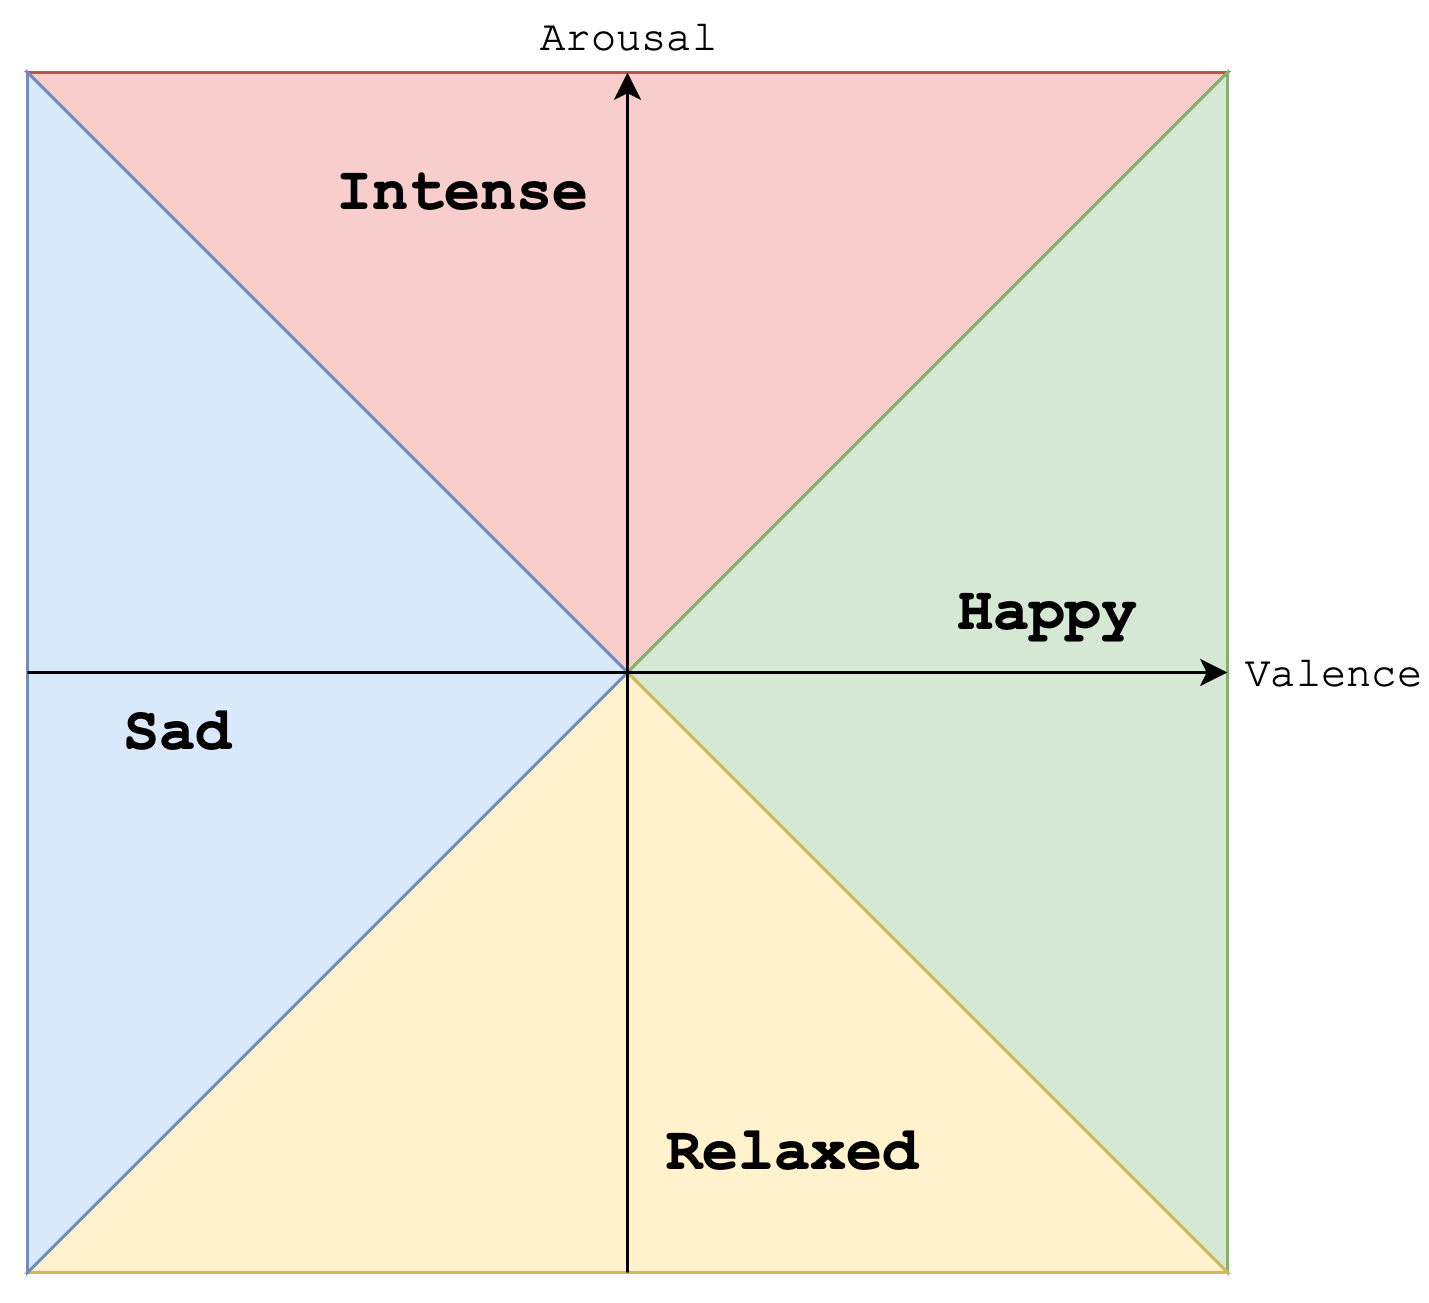
\includegraphics{Images/circumplex.png}
\caption{Two dimensional representation of the Circumplex model with
labels plotted on the resulting plane}
\end{figure}

In this context, arousal refers to the perceived intensity of a piece;
ranging from a relaxed or somewhat lethargic feeling to a more intense
and excited stimulation. Valence is a spectrum of the affect on a
listeners level of happiness or sadness which may be incited by the
piece. Values for both axes were estimated and ratios calculated to
fulfil three ratio values regarding each axis. The ratios are calculated
as shown below following predictions made by the models:

\[\begin{aligned}
S_A &= \{\text{Scores assigned to each input by the arousal regressor model}\} \\
\text{Arousal Intense Ratio } &= \frac{\sum_{S_A} \mathbbm{1}_{\text{Score}> 2}}{|S_A|} \\
\text{Arousal Relaxing Ratio } &= \frac{\sum_{S_A} \mathbbm{1}_{\text{Score}< 1}}{|S_A|} \\
\text{Arousal Mid Ratio } &= 1 - (\text{Arousal Intense Ratio} + \text{Arousal Relaxing Ratio}) \\ \\
S_V &= \{\text{Scores assigned to each input by the valence regressor model}\} \\
\text{Valence Happy Ratio } &= \frac{\sum_{S_V} \mathbbm{1}_{\text{Score}> 2}}{|S_V|} \\
\text{Valence Sad Ratio } &= \frac{\sum_{S_V} \mathbbm{1}_{\text{Score}< 1}}{|S_V|} \\
\text{Valence Neutral Ratio } &= 1 - (\text{Valence Happy Ratio} + \text{Valence Sad Ratio}) \\
\end{aligned}\]

In both cases it can be seen that ratios are calculated through taking
the top and bottom few scores and calculating the ratio of each above
and below boundaries which were formulated through testing and with
respect to the original work. It is worth noting that all scores fall
between a range of 0 and around 5, but extreme values are clipped to 3
as they do not appear and are often spurious.

\hypertarget{implementing-signal-processing-technique-and-returning-the-results-in-a-usable-form}{%
\subsection{Implementing Signal Processing Technique and Returning the
Results in a Usable
Form}\label{implementing-signal-processing-technique-and-returning-the-results-in-a-usable-form}}

Most of the code relevant to this section is included in the
\texttt{mood.py} file included with this document.

Each piece to be analysed is trimmed of its start and end (which are
likely to be sparse and potentially irregular in terms of their content
when compared to the main body of a piece occurring around its midpoint)
to leave the middle 70\% of the data. This raw data is then windowed
into 5-second long frames of samples, with a step of 0.5 seconds between
the starting points of each (such that there is overlap between frames).
Within each of these there is then a further decomposition into 25ms
sub-frames that are transformed into an array of Mel-frequency cepstral
coefficients (MFCCs). The matrices representing the coefficients for
each sub-frame are then flattened and fed into a 3-layer neural network
regressor. The neural networks associate patterns common within certain
moods based upon what was learnt from numerous large datasets used for
training these models.

ADD DIAGRAM? HARD

These ratios are then packed into a 6 item vector and associated with
each of the training MIDI files to be loaded during training.
Thresholding as a means of segmentation was implemented by setting all
ratios greater than 50 to 1 and those below 50 to 0. This offered
computational improvements but slightly decreased the effectiveness of
the mood transfer to training pieces in the opinion of the author and
some survey participants. Due to the subjectivity of this part of the
output, it was hard to assess which approach was more effective in
capturing mood and so the simpler, less computationally intense
thresholding option was chosen. This resulted in a six element
\emph{binary} vector representing mood associated with each item in the
training corpus.

\hypertarget{creating-a-recurrent-model-for-musical-composition}{%
\section{Creating a Recurrent Model for Musical
Composition}\label{creating-a-recurrent-model-for-musical-composition}}

\hypertarget{recurrent-neural-networks}{%
\subsection{Recurrent Neural Networks}\label{recurrent-neural-networks}}

Perhaps the most common form of artificial neural network is the
\emph{feedforward} network which utilise connected layers of neurons and
activation functions to approximate different functions through the
learning of parameters and weights. Their main limitation in this
context is that they require their inputs to be of a fixed dimension and
thus are not well suited to dynamic data of varying size such as a
sequence \((x_t)_{1\le t\le T}\) of time stepped note states
representing a composition where \(T\) is the length of the piece.

It is assumed that this type of sequential data has some system of
dependence on its prior and potentially future elements and so it would
not be appropriate to assume independence and simply input each element
of a temporal sequence into a feedforward network during training. It
can clearly be seen by observing musical data and considering knowledge
of musical theory that the input at each time step is likely to be
dependent on other time steps (compositions have an associated and
consistent \emph{key} which may be inferred by chords and notes present
throughout the piece).

This class of situations led to the development of \textbf{Recurrent
Neural Networks} which introduce recurrent connections between layers
over a temporal dimension allowing the network to exhibit dynamic
behaviour over time. Their evolution over time depends on the inputs as
well as its previous / current state. They could be considered to be an
evolution of Hidden Markov Models
{[}\protect\hyperlink{ref-baum1966}{34}{]} but with the addition of a
distributed state allowing for more complex and dynamic behaviours to be
captured in a computationally effective manner.

It is now possible to provide some notation specific to this project
regarding RNNs. A training input is defined
\protect\hyperlink{buildinganeffectiverepresentation}{as before}, with
the vector corresponding to the sequence at time \(t\) denoted as
\(x_t\in \{0,1\}^{D_{\text{input}}}\). At each time step, a layer's
input \(x_t\) and its previous state \(h_{t-1}\) are used to calculate a
new value \(h_t\) for each hidden layer \(h\in\{\text{Hidden Layers}\}\)
and also inform the outputs for that time step \(y_t\). Mathematically,
this relationship is as follows:

SOURCE, ALSO SHOULD I TALK MORE ABOUT BACK PROP AND HOW IT ACTUALLY
LEARNS, DONT WANT TO COMPLETELY REWRITE RNN PAPERS HAHA

\[\begin{aligned}
h_t &= \phi(W_{xh} x_t + W_{hh} h_{t-1} + b_{xh}) \\
y_t &= W_{hy}(h_t) + b_{hy}
\end{aligned}\]

Where:

\begin{itemize}
\tightlist
\item
  \(\phi\) is the chosen element-wise activation function for the
  network
\item
  \(W_{xy}\) represents the weight parameters between layers \(x\) and
  \(y\), these weight parameters are learned using backpropagation
  through time
  {[}\protect\hyperlink{ref-werbos1990backpropagation}{35}{]}
\item
  \(b_{xy}\) is the bias parameter between layers \(x\) and \(y\)
\end{itemize}

In this case and all proceeding cases, where there are multiple hidden
layers, assume that the input for the \(n^{\text{th}}\) layer
\(h^{(n)}_t\) is \(x_t = h^{(n-1)}_t\).

\begin{figure}
\centering
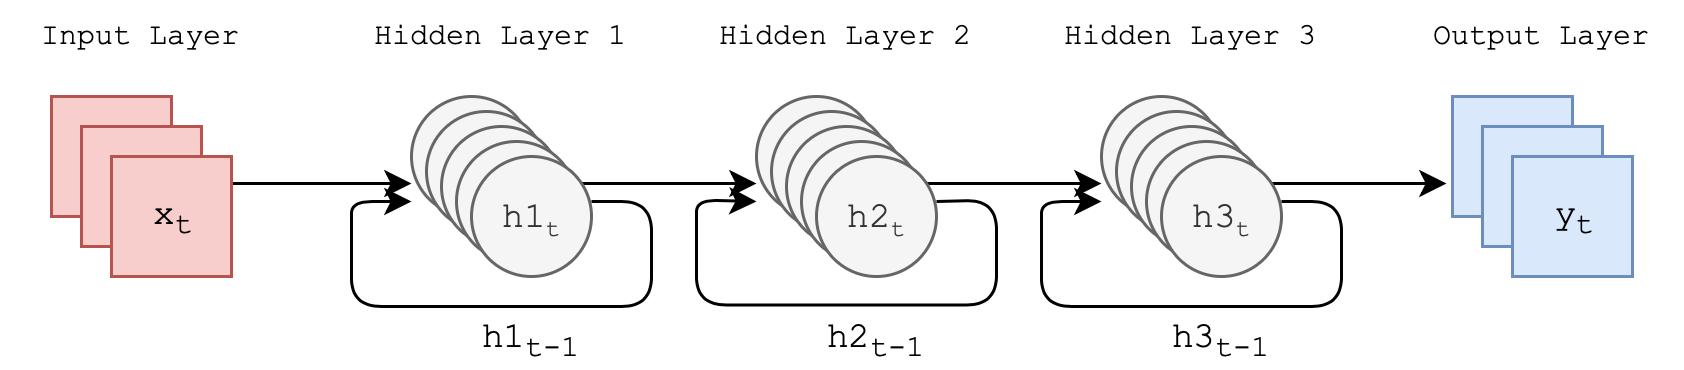
\includegraphics{Images/rnn.png}
\caption{Recurrent connections between the hidden layers of a network}
\end{figure}

This process is illustrated in the figure above and can be described by
considering that at the start of the process all weights and activations
are initialised to some value. At each time step following this, the new
activations for each hidden layer are calculated using a combination of
the current time step's input and that layer's previous activations.
This process highlights the possibility of unrolling an RNN into a DAG
representation as shown in the figure below.

\begin{figure}
\centering
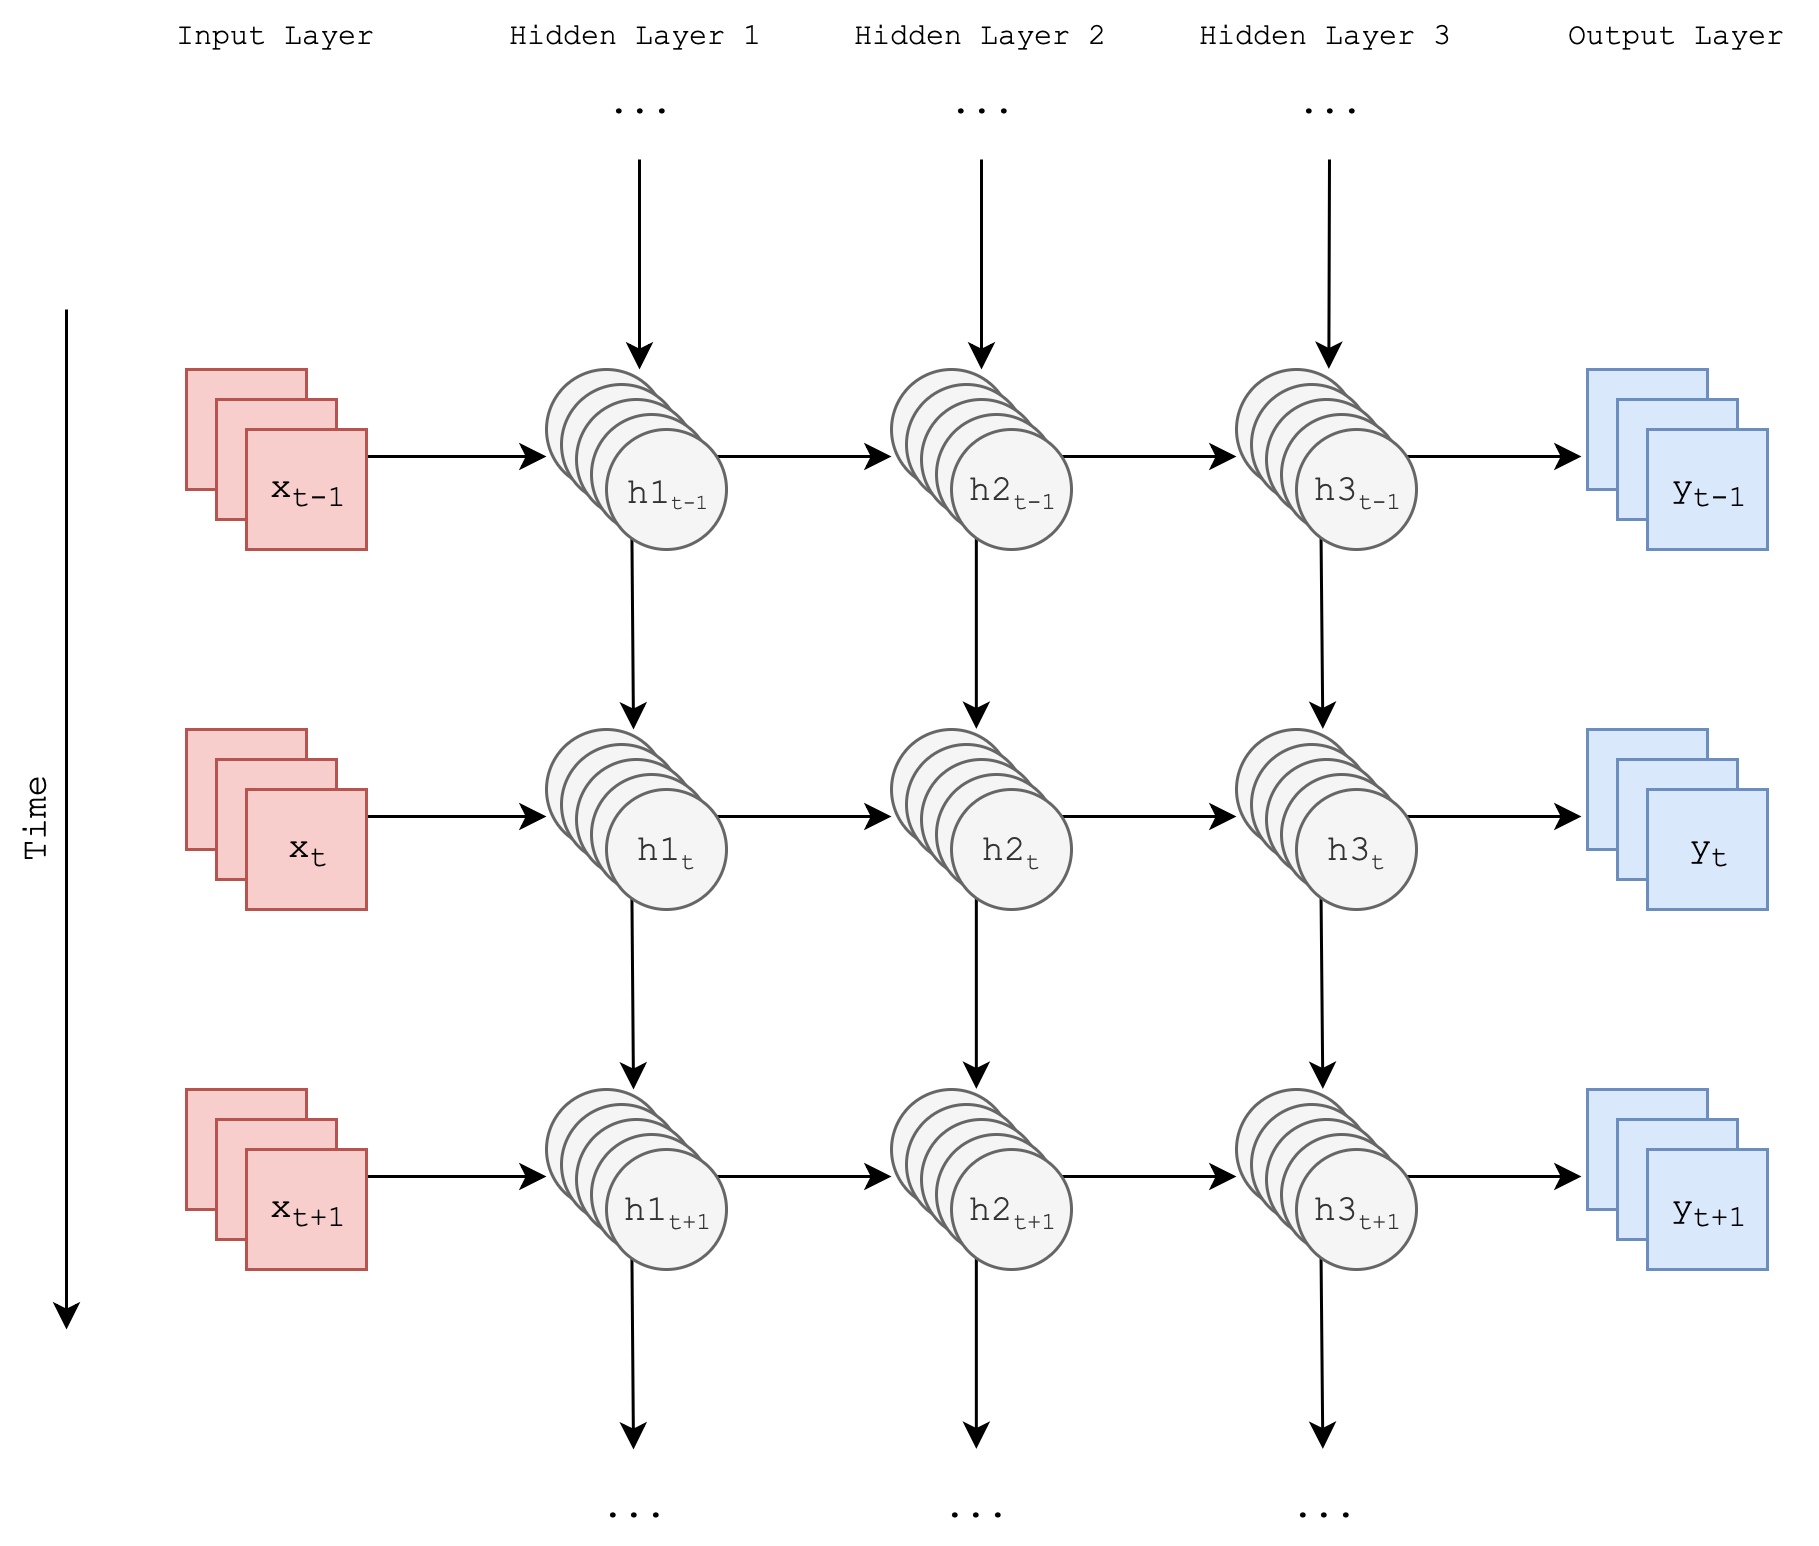
\includegraphics{Images/unrolledrnn.png}
\caption{Identical to the previous figure in meaning but with the
recurrent connections unrolled along the time axis}
\end{figure}

The potentially most important property of this class of networks is
their \emph{time invariance}, in that at a given time step the networks
activations and learned properties can all be considered relative to
previous time steps. The activations at one time step influence the next
and potentially all future time steps moving forward, meaning
dependencies can be learned over time. The ability to recurrently input
data into the network is the clear reason for its usage in this context
over traditional feedforward networks.

Despite this time invariance and flexibility in terms of the dimension
of their inputs, they lack long term coherence meaning they often fail
when complex dependencies are built up and different temporal structures
must be captured. They are susceptible to exploding or vanishing
gradients over time due to repeated and recurrent backpropagation,
i.e.~tiny values will often compound and be multiplied together leading
to the network getting stuck or significantly slowing its learning.
These issues have inspired a number of variants aiming to mitigate these
problems and form the basis of most current approaches to musical
composition. Through considerable research, it was decided that LSTMs
and GRUs should be trialled against each other as part of this project's
model architecture. They are both discussed in the sections below.

\hypertarget{issues}{%
\subsubsection{Issues}\label{issues}}

\hypertarget{long-short-term-memory-recurrent-units}{%
\subsubsection{Long Short-Term Memory Recurrent
Units}\label{long-short-term-memory-recurrent-units}}

The LSTM unit was first proposed in 1999
{[}\protect\hyperlink{ref-gers1999learning}{36}{]}, though the version
formulated here includes some improvements based on more recent research
{[}\protect\hyperlink{ref-sak2014long}{37}{]}--{[}\protect\hyperlink{ref-zebin2018human}{39}{]},
the most notable addition is that of the \emph{forget gate}. LSTMs
introduce a means of allowing long-term dependencies to be captured by
RNNs through introducing three `gates' which each interact with a memory
state and previous hidden activations passed through time:

\begin{itemize}
\tightlist
\item
  The \textbf{forget gate} is a scaling factor
  \[f_t = \sigma(W_{if} x_t + b_{if} + W_{hf} h_{(t-1)} + b_{hf})\]
  where \(\sigma(x) = 1 / (1 + e^{-x})\) is the sigmoid function; its
  values fall in \([0,1]\) and control the extent to which the previous
  cell memory state \(c_{t-1}\) is kept
\item
  The \textbf{input gate} is a scaling factor
  \[i_t = \sigma(W_{ii} x_t + b_{ii} + W_{hi} h_{(t-1)} + b_{hi})\]
  where the terms are self-explanatory; its values fall in \([0,1]\) and
  control the extent to which the new input \(x_t\) flows into the unit
\item
  The \textbf{output gate} is a scaling factor
  \[o_t = \sigma(W_{io} x_t + b_{io} + W_{ho} h_{(t-1)} + b_{ho})\]
  where the terms are self-explanatory; its values fall in \([0,1]\) and
  control the extent to which the new candidate memory state \(c^*_t\)
  is used to compute the new activation \(h_t\)
\end{itemize}

The candidate memory state \(c^*_t\) is calculated as
\[c^*_t = \tanh(W_{ic^*} x_t + b_{ic^*} + W_{hc^*} h_{(t-1)} + b_{hc^*})\]
which can then be multiplied element-wise with the input gate scaling
factor and added with the result of the forget gate scaling factor's
element-wise multiplication with the previous memory state:
\[c_t = f_t \odot c_{t-1} + i_t \odot c^*_t\] Finally, the new / current
hidden activation state can be found as: \[h_t = o_t \odot \tanh(c_t)\]
All of these weights and bias parameters are updated during training via
backpropagation as before and initialised in this instance from the
uniform distribution:
\[U(-\sqrt{k}, \sqrt{k}),\quad k = \frac{1}{\text{Hidden Layer Size}}\]

The diagram below illustrates the LSTM and the flow of data through it
diagrammatically.

\begin{figure}
\centering
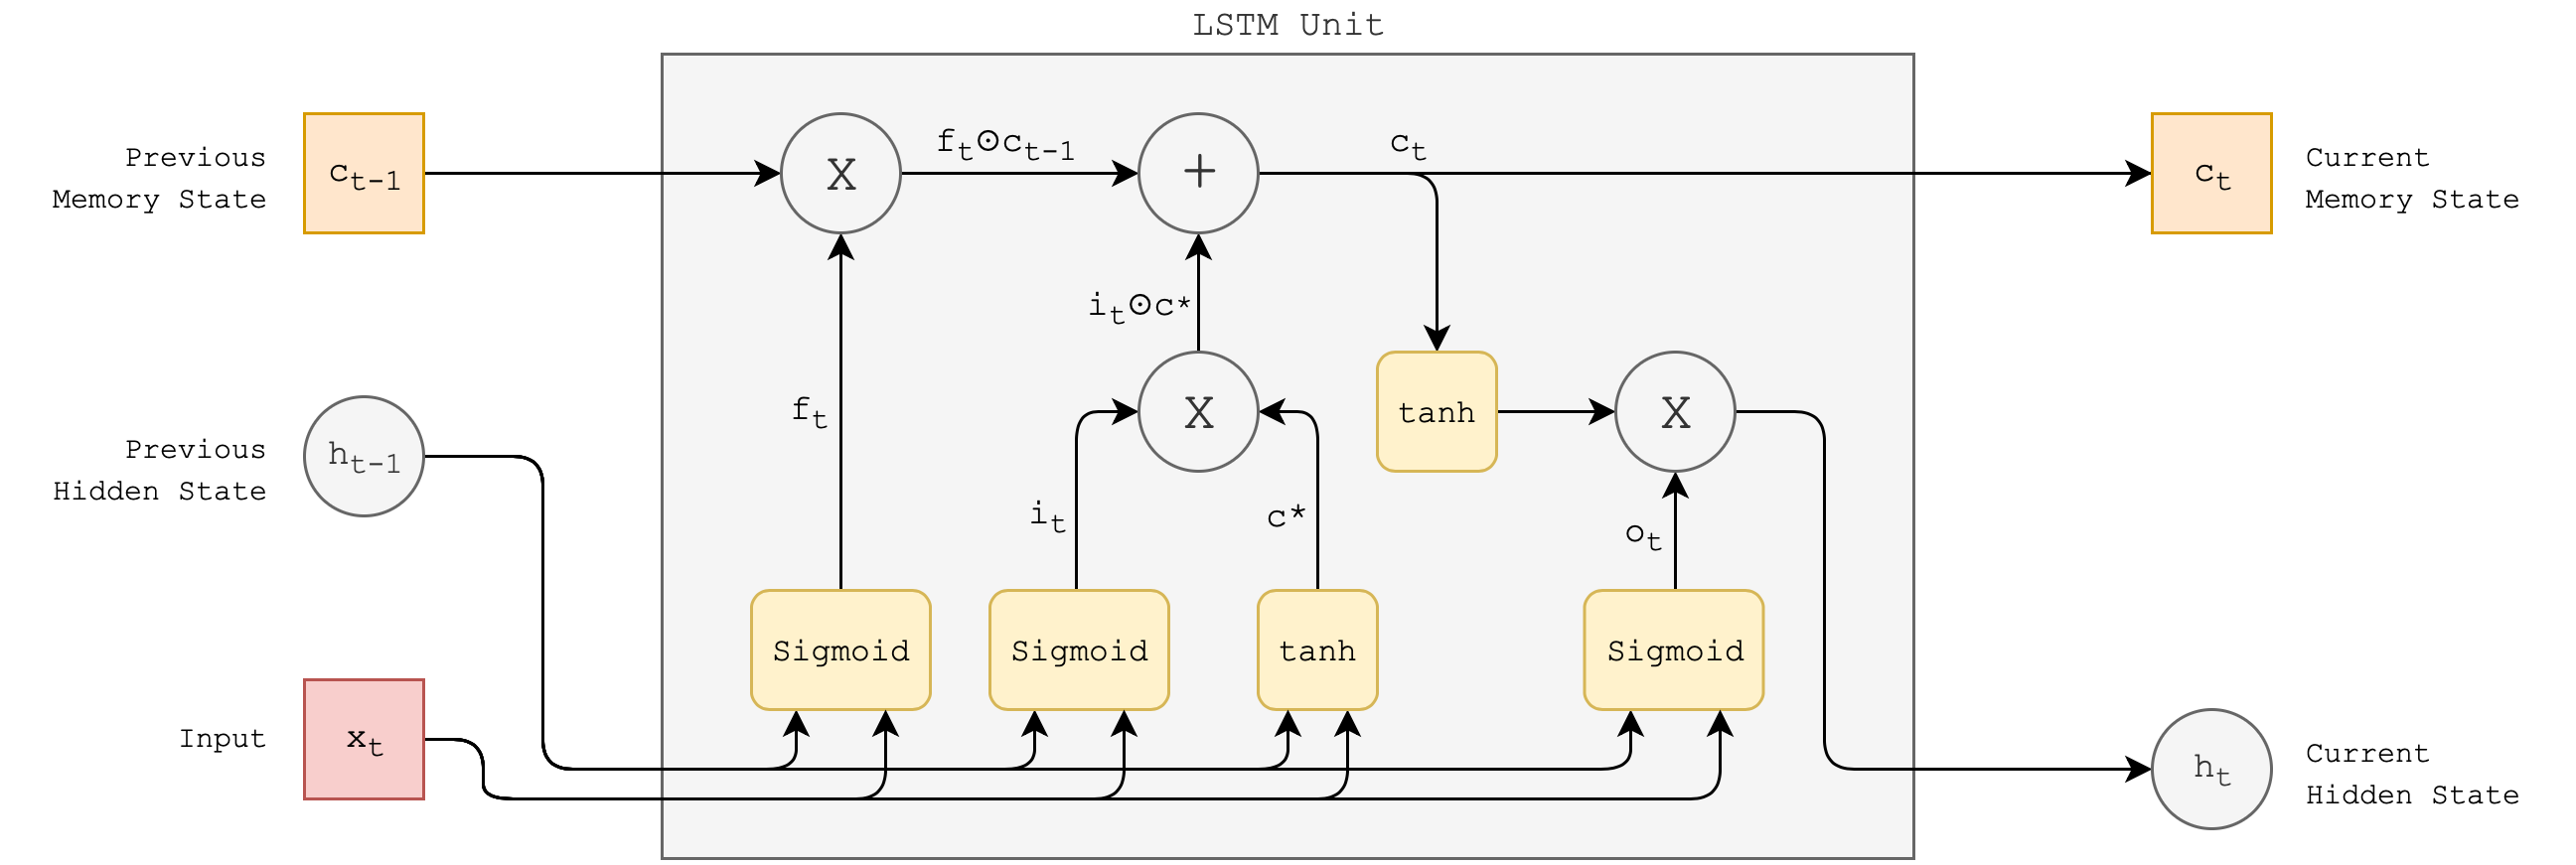
\includegraphics{Images/lstm.png}
\caption{A single Long Short-Term Memory Unit taking input at a single
time step}
\end{figure}

Note that there are many small variations on the LSTM concept; the
mathematical formulation was written here in context of PyTorch's
implementation {[}\protect\hyperlink{ref-pytorchlstm}{40}{]} and the
figure reflects this.

\hypertarget{gated-recurrent-units}{%
\subsubsection{Gated Recurrent Units}\label{gated-recurrent-units}}

The GRU was first proposed in 2014 {[}cho2014learning{]}. It offers a
similar set of operations to try and mitigate the aforementioned issues
with RNNs. It does so by introducing two `gates' in a slightly simpler
configuration to the LSTM:

\begin{itemize}
\tightlist
\item
  The \textbf{reset gate} is a scaling factor
  \[r_t = \sigma(W_{ir} x_t + b_{ir} + W_{hr} h_{(t-1)} + b_{hr})\]
  where \(\sigma(x) = 1 / (1 + e^{-x})\) is the sigmoid function; its
  values fall in \([0,1]\) and control the extent to which the previous
  cell memory state \(c_{t-1}\) is kept
\item
  The \textbf{update gate} is a scaling factor
  \[z_t = \sigma(W_{iz} x_t + b_{iz} + W_{hz} h_{(t-1)} + b_{hz})\]
  where the terms are self-explanatory; its values fall in \([0,1]\) and
  control the extent to which the unit's activation is updated
\end{itemize}

The candidate activation state \(h_t^*\) is calculated as
\[h_t^* = \tanh(W_{ih^*} x_t + b_{ih^*} + r_t (W_{hh^*} h_{(t-1)} + b_{hh^*}))\]
which can then be used in calculating the new / current activation via a
linear interpolation of the candidate activation and the previous
activation: \[h_t = h_{t-1} (1 - z_t) + h_t^* z_t\]

The diagram below illustrates the GRU and the flow of data through it
diagrammatically.

\begin{figure}
\centering
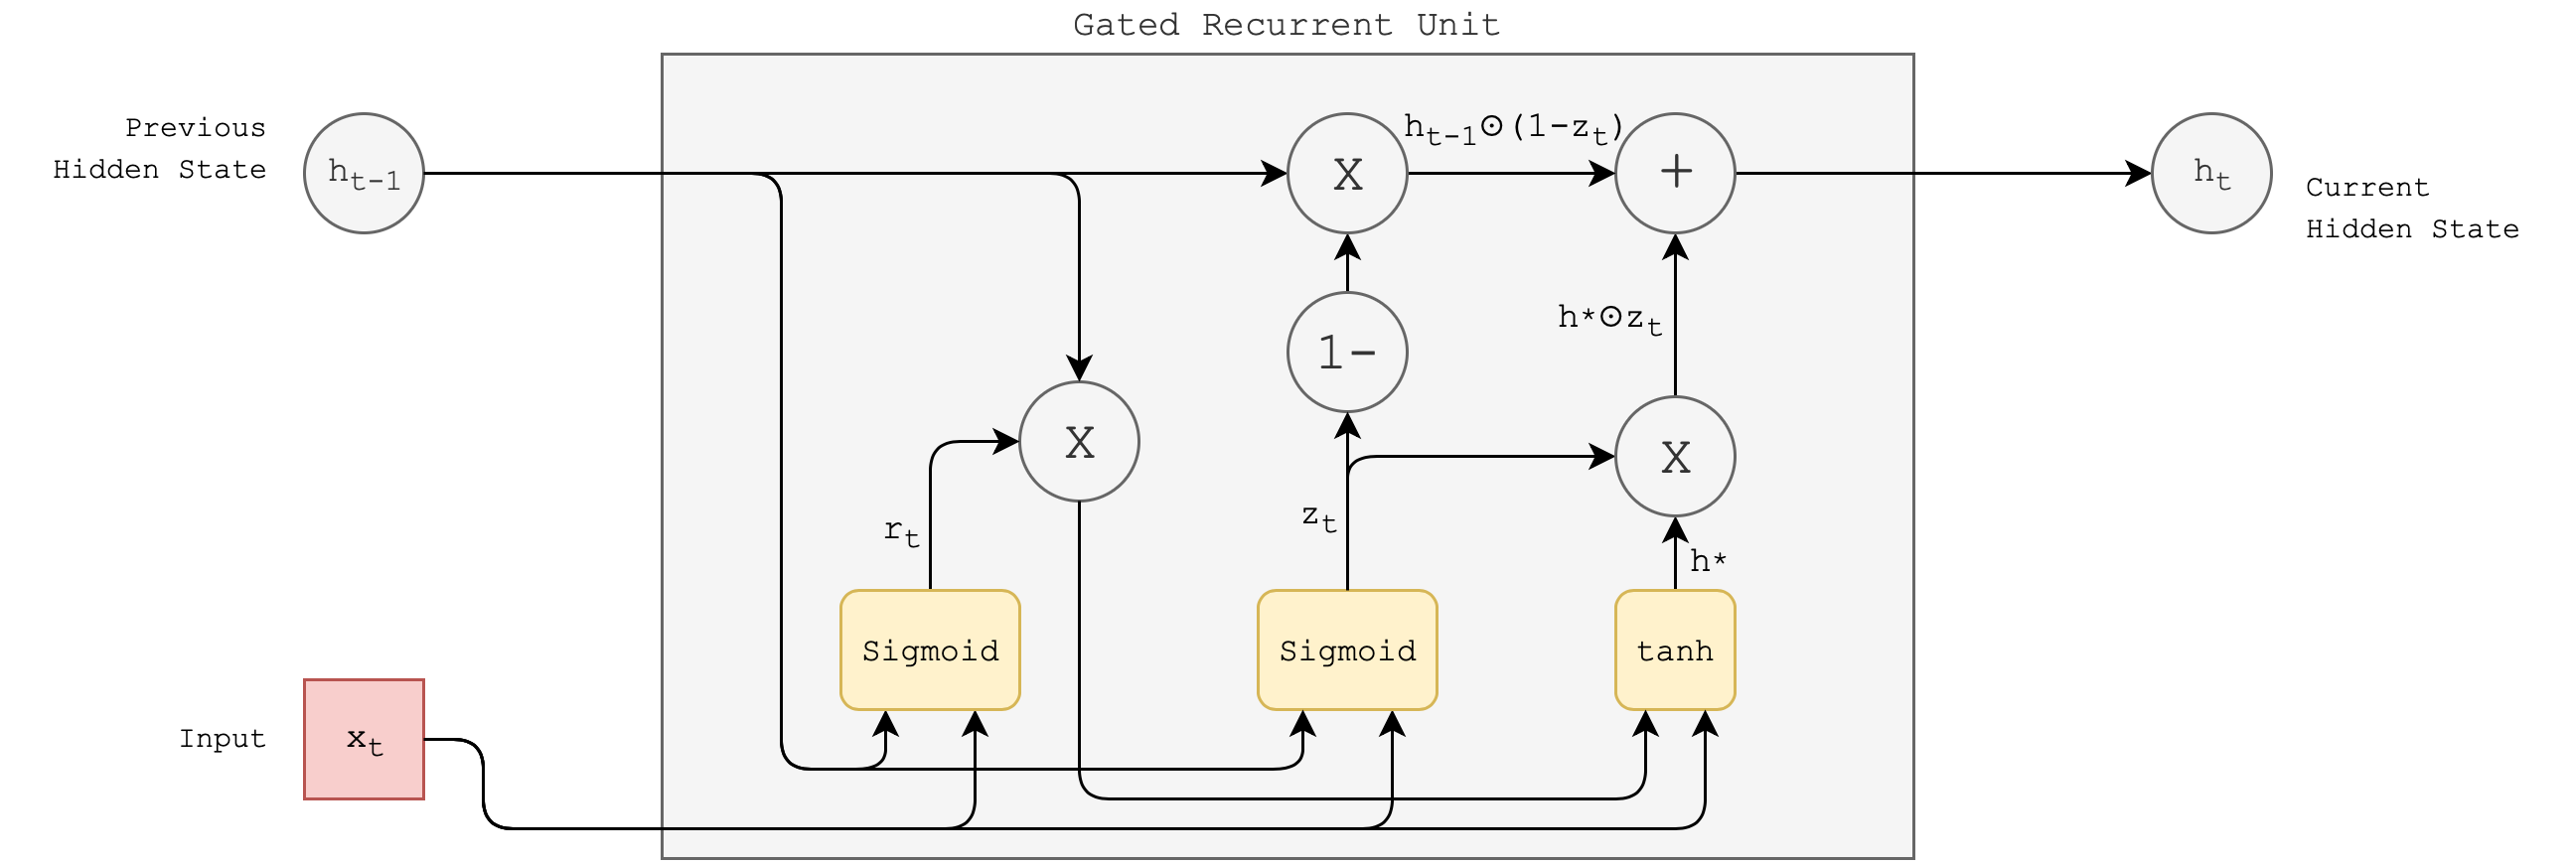
\includegraphics{Images/gru.png}
\caption{A single Gated Recurrent Unit taking input at a single time
step}
\end{figure}

Note that there are many small variations on the GRU concept; the
mathematical formulation was written here in context of PyTorch's
implementation {[}\protect\hyperlink{ref-pytorchgru}{41}{]} and the
figure reflects this.

\hypertarget{dilation}{%
\subsection{Dilation}\label{dilation}}

The concept of dilation was first proposed in the context of
convolutional neural networks
{[}\protect\hyperlink{ref-yu2015multi}{42}{]} for image analysis and
semantic segmentation; this work was discovered during research for a
\protect\hyperlink{sentimentalinputfromimages}{potential extension} of
this project. The main concept is to aggregate information at different
contextual scalings without losing resolution by exploding a kernel's
considered neighbourhood around a central pixel / element. This is done
to increase the likelihood of discovering pattern structures at
different resolutions within an input as well as increasing the area of
an image or input which can be considered through a small number of
steps.

It offers an alternative to other techniques often relying on
down-sampling which sacrifice resolution rather than considering
different contexts at full resolution as is the case with dilation.

\begin{figure}
\centering
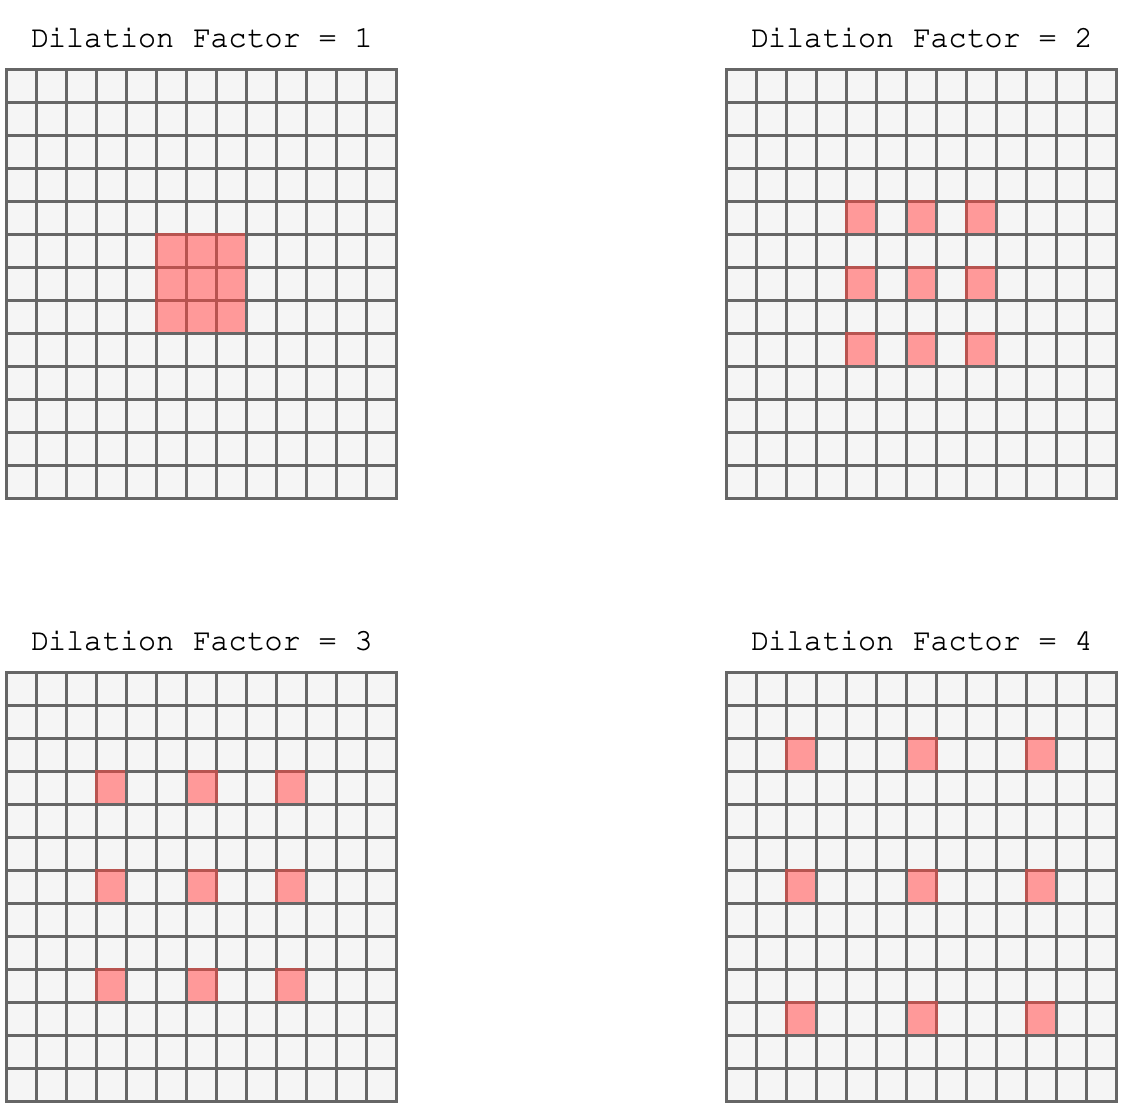
\includegraphics[width=0.7\textwidth,height=\textheight]{Images/dilation2d.png}
\caption{Different dilation factors (represented by the value of D)
illustrated on a 2-dimensional input}
\end{figure}

This technique has shown to be very effective in aiding dense prediction
problems (predicting labels for each pixel in an image, or with respect
to this project's proposed equivalence of predicting on or off states
for each note on the piano over a series of time steps). Deepmind
researchers applied a similar approach within their own convolutional
network for WaveNet which is the first documented use of dilation in the
musical composition domain
{[}\protect\hyperlink{ref-oord2016wavenet}{21}{]}. Their results found
that again the addition of dilation increased the accuracy and
effectiveness of their model.

A paper was published linking this concept with recurrent neural
networks in 2017 {[}\protect\hyperlink{ref-chang2017dilated}{43}{]}.
This paper forms the basis for the justification of using dilation in
the model present in this project; this project's compositional model is
potentially the first use of dilated recurrent neural networks in the
musical composition domain. Dilation's purpose in this context is to
allow a model to learn at multiple temporal resolutions and capture the
complexities of musical composition that exist naturally through its
formulation in terms of half and double length notes, beats, bars etc.
This immediately lends itself to dilation POWERS OF 2.

\begin{figure}
\centering
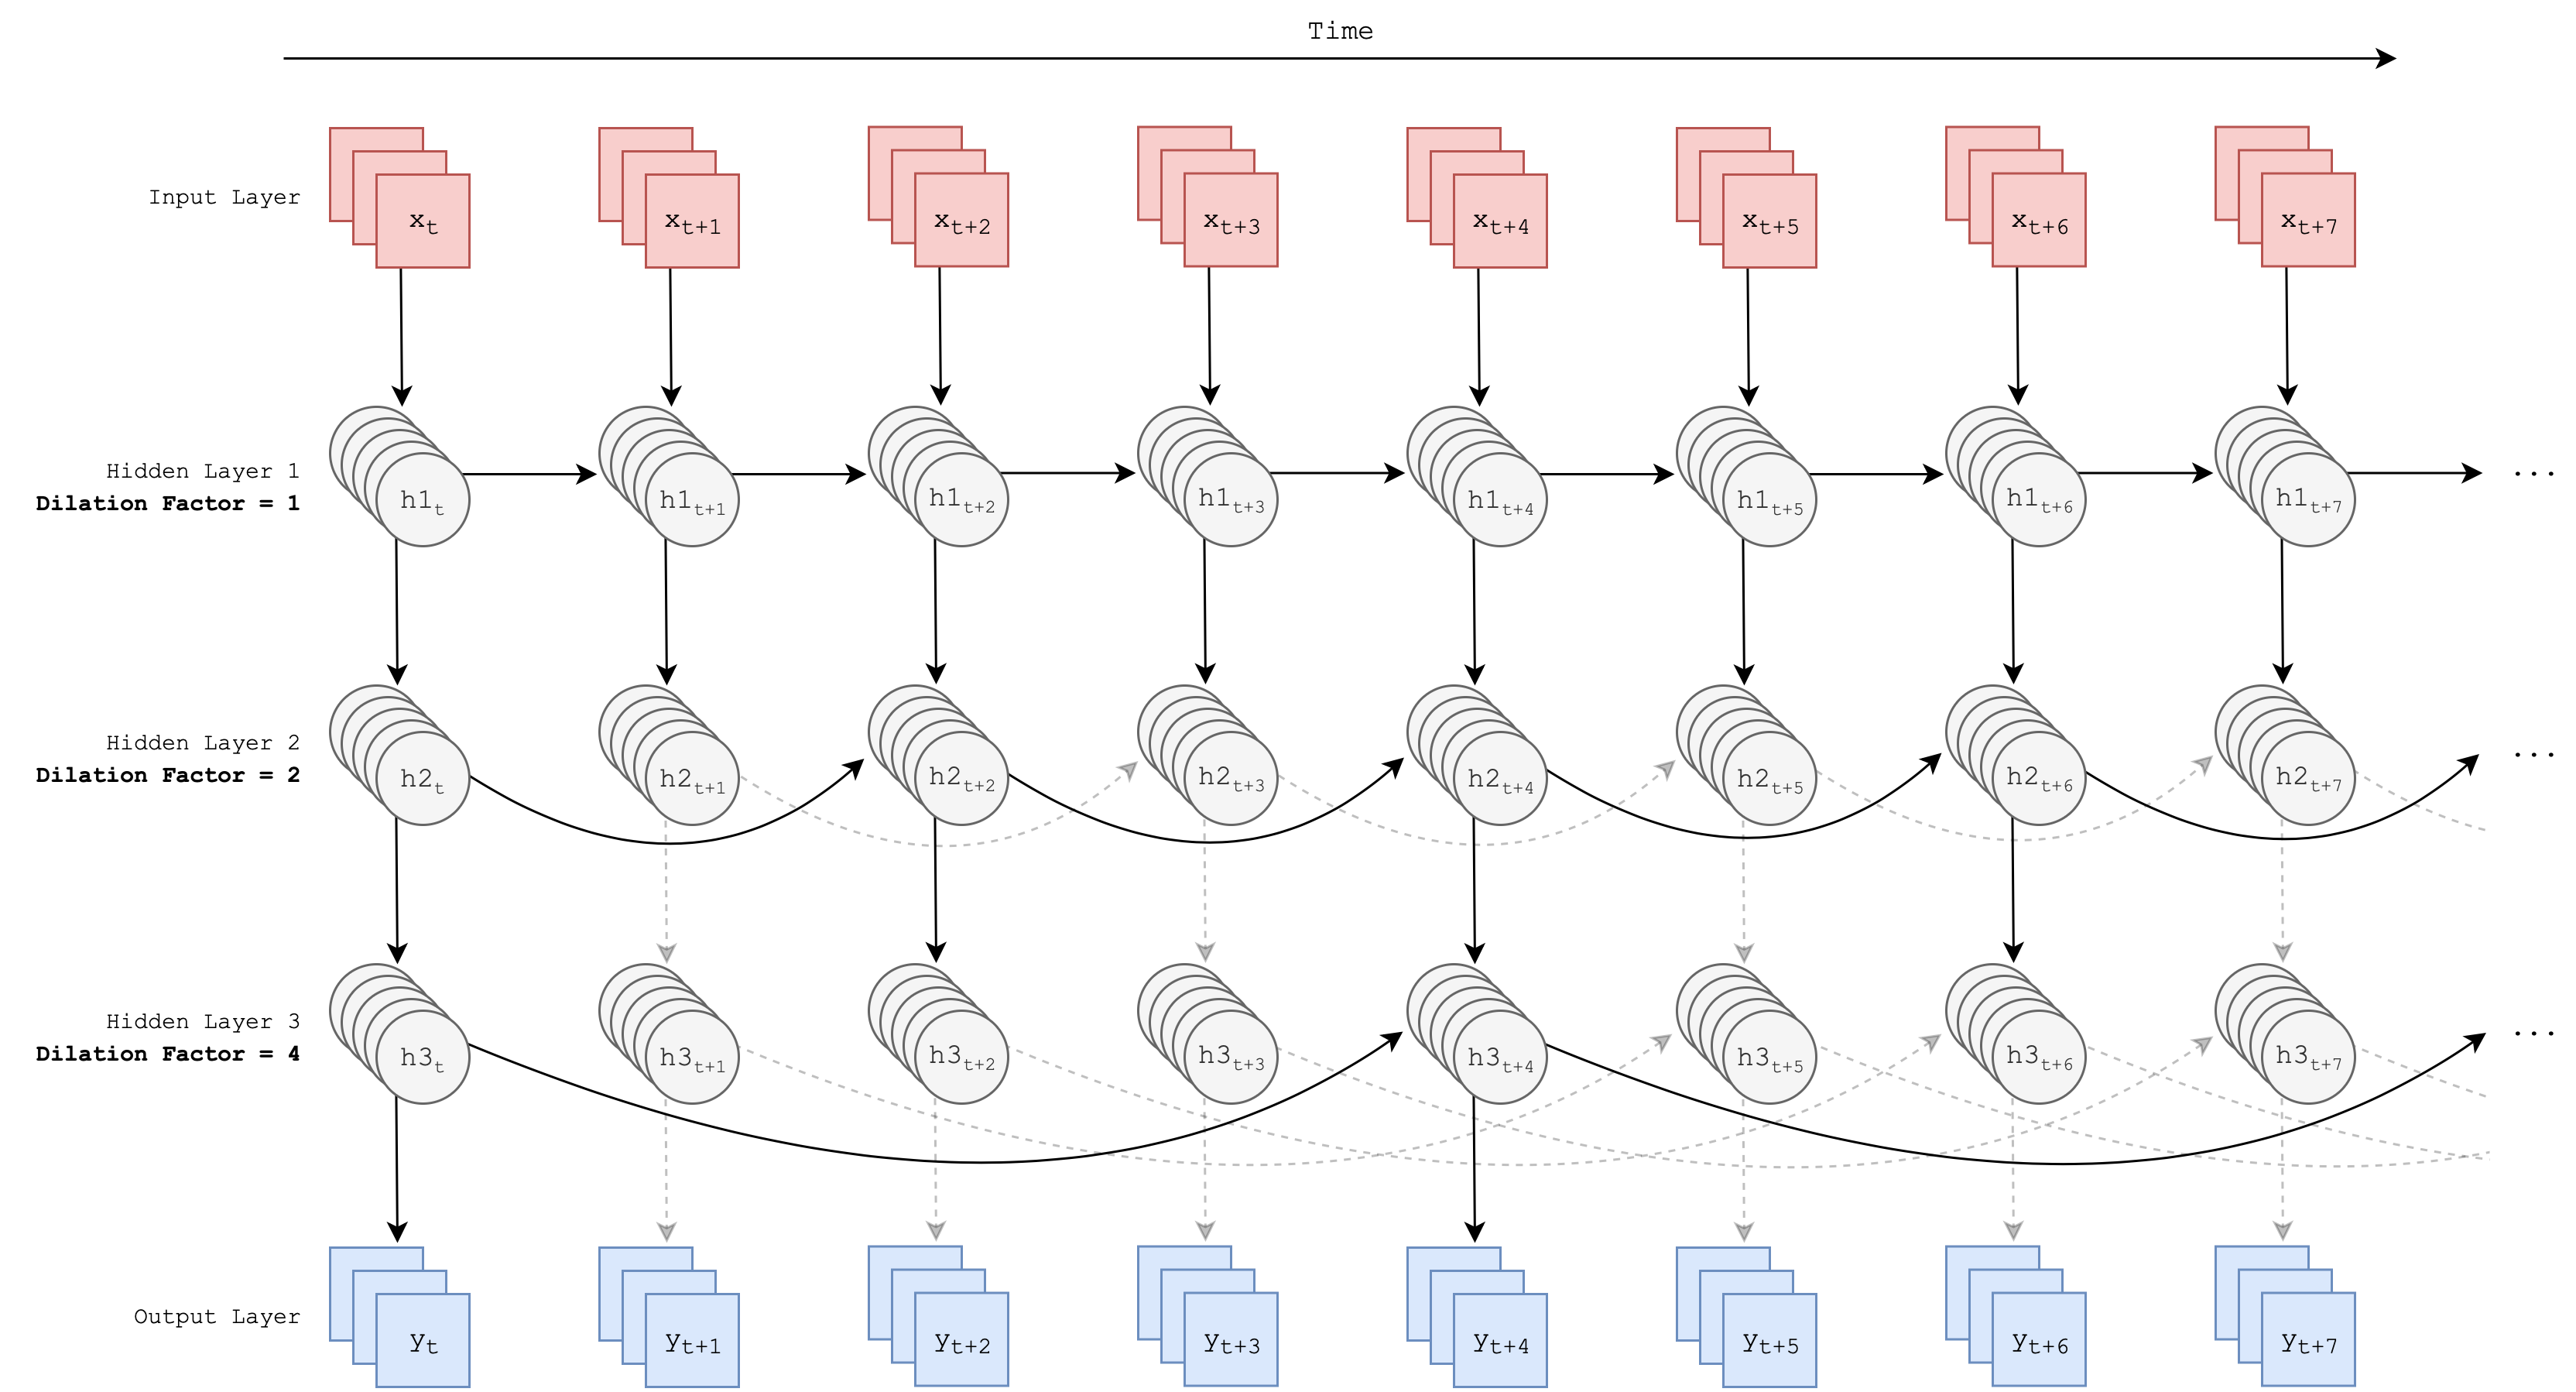
\includegraphics[width=1\textwidth,height=\textheight]{Images/dilatedrnn.png}
\caption{An example of a three-layer DRNN with dilation factors 1, 2,
and 4}
\end{figure}

\begin{figure}
\centering
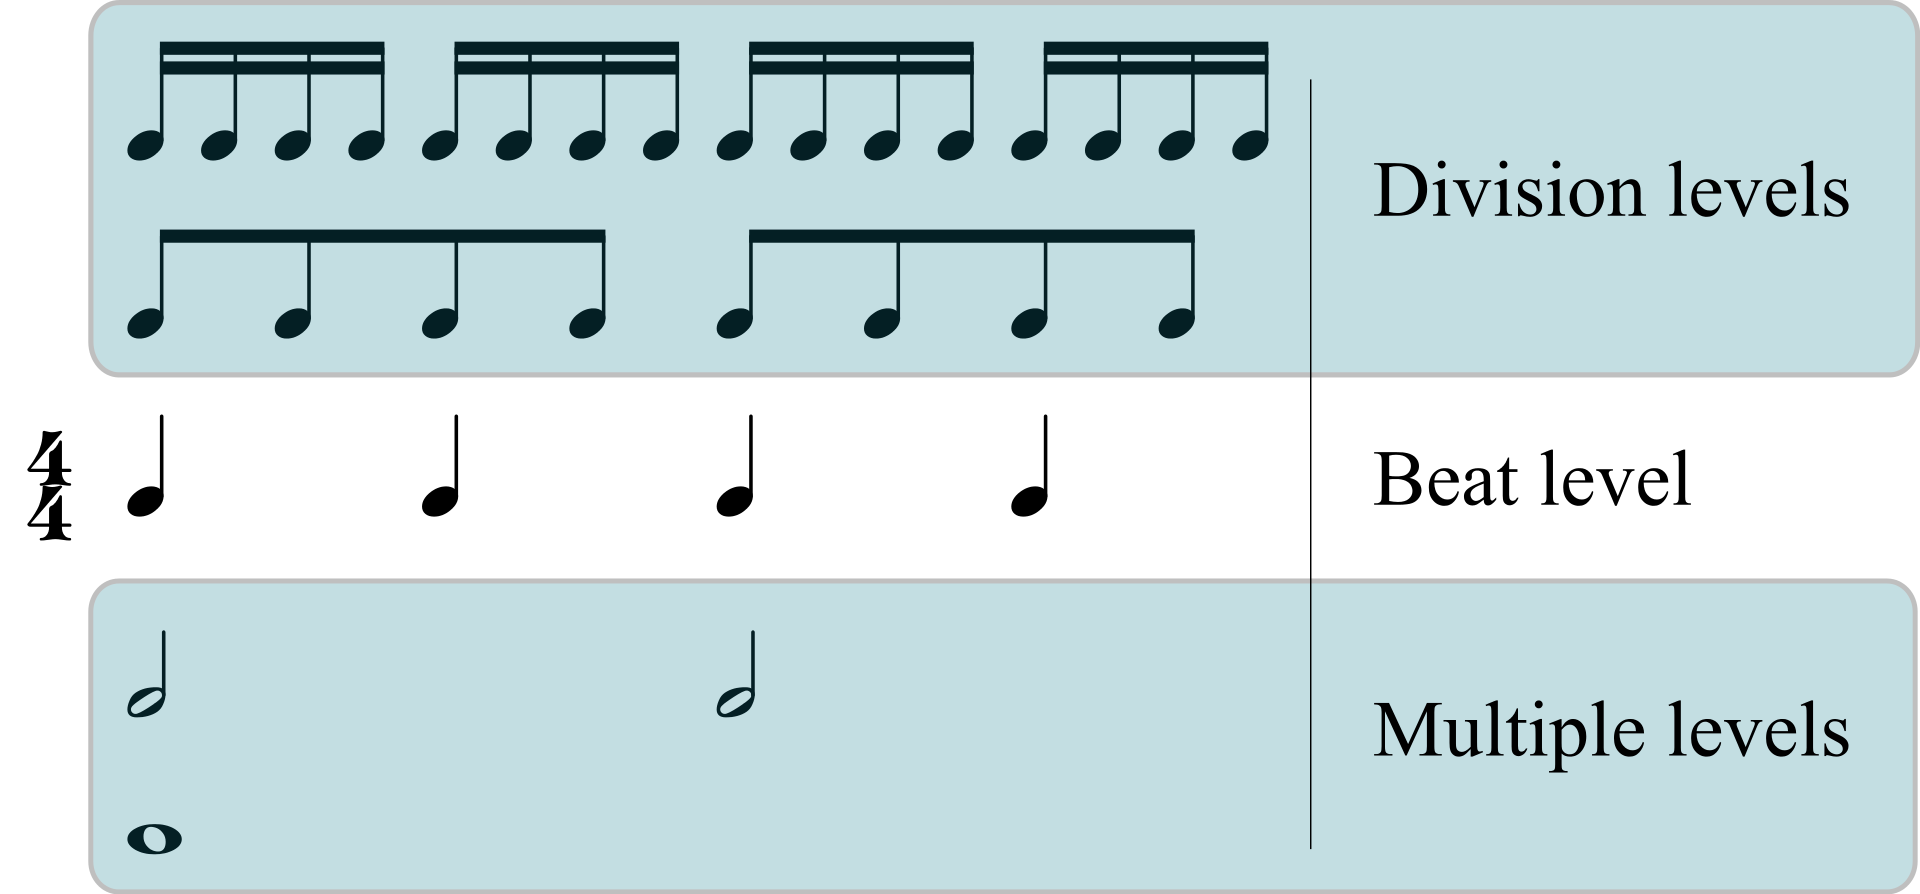
\includegraphics[width=0.7\textwidth,height=\textheight]{Images/Metric_levels.png}
\caption{The parallels between musical temporal structure and a DRNN's
structure are clear}
\end{figure}

Mathematically, dilation can be achieved by simply reconnecting the
network's layers such that all of the aforemenetioned recurrent
operations are done with respect to \(t-D_l\) rather than \(t-1\) where
\(D_l\) is the dilation factor of layer \(l\). Enhanced parallelisation
can be achieved by computing dilated layers together at the same time as
illustrated below:

\begin{figure}
\centering
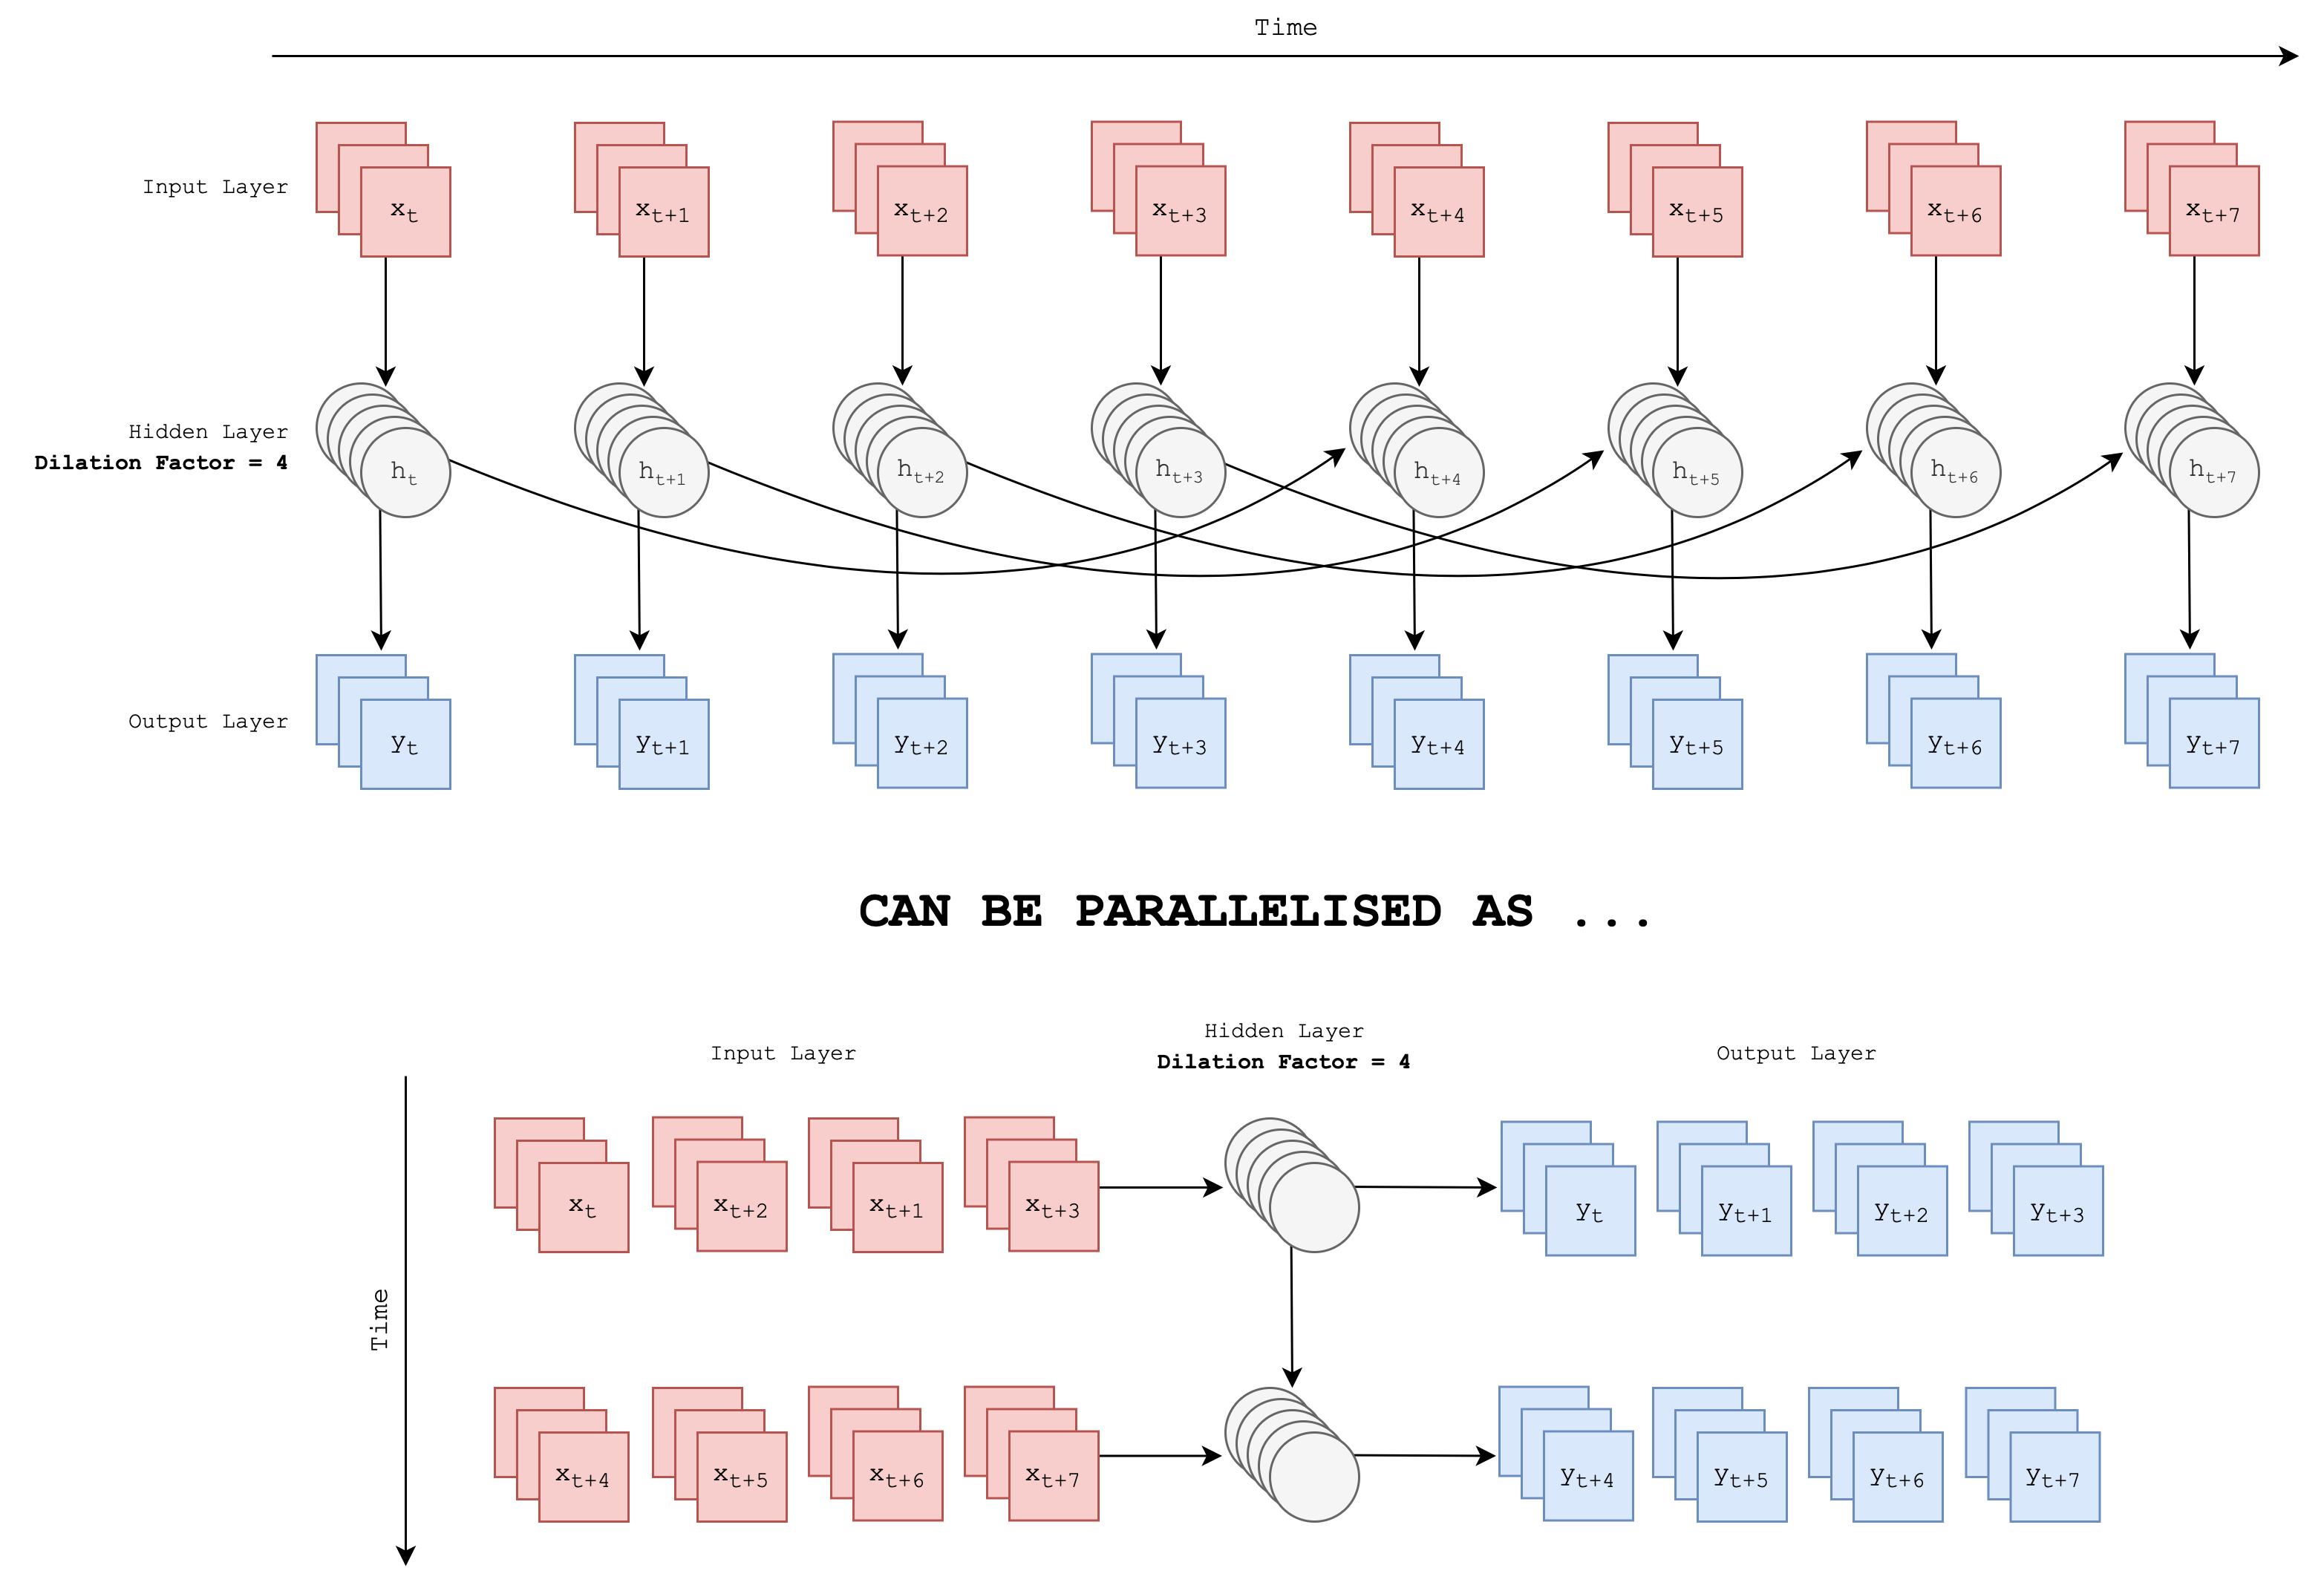
\includegraphics{Images/dilatedrnnparallel.png}
\caption{The four chains of recurrent units shown at the top of this
diagram can be computed in parallel rather than at separate time steps,
as all of them occur across the same distance in time, this can have
huge performance implications where parallel computation is enabled such
as when utilising GPUs to train a model}
\end{figure}

\hypertarget{introducing-harmonic-invariance}{%
\subsection{Introducing Harmonic
Invariance}\label{introducing-harmonic-invariance}}

The consideration of musical theory is the main inspiration for the
following section. There is a large body of documentation and research
surrounding musical theory which a reader could investigate should they
wish to supplement this paper with additional context. However, the
essentials and relevant points are included for convenience.

In general, compositions are written with respect to a \textbf{key}
which roughly determines the scales upon which harmonics and chords for
a piece are constructed. Each key is simply a transformation or rather a
transposition of another through some number of shifts up or down.

\begin{figure}
\centering
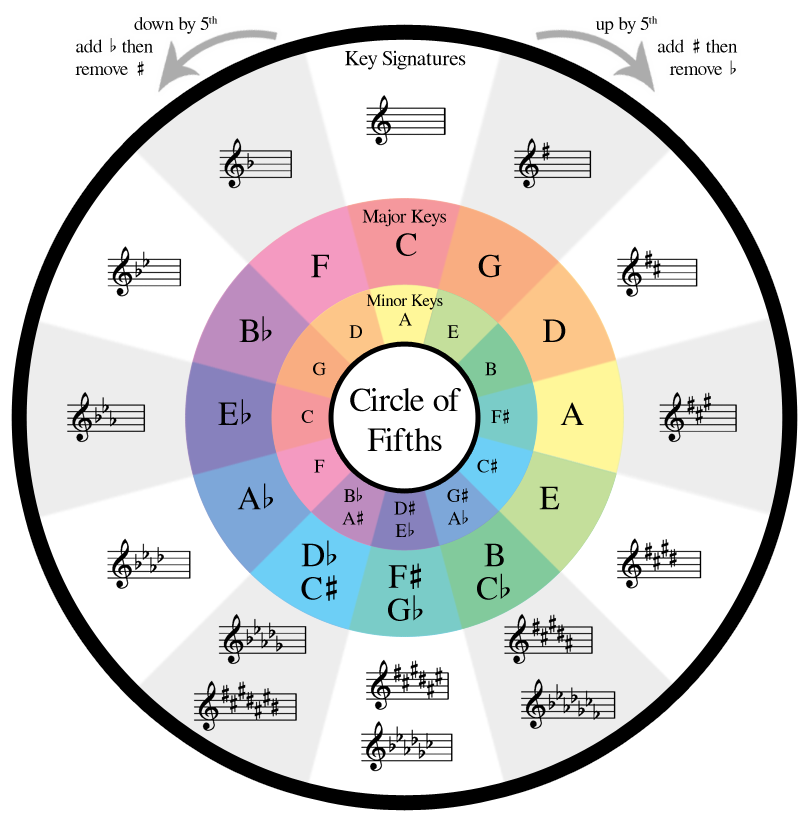
\includegraphics[width=\textwidth,height=0.4\textheight]{Images/flypaperfifths.png}
\caption{Diagram illustrating the Circle of Fifths, note that going up
by a 5th (5 notes) is equivalent to going down by 4 notes and vice
versa. Source: FlyPaper}
\end{figure}

\begin{figure}
\centering
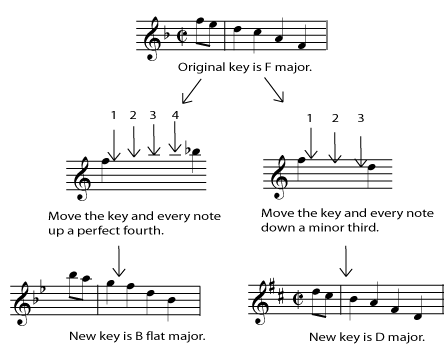
\includegraphics[width=\textwidth,height=0.3\textheight]{Images/transp3b.png}
\caption{Example of a transposition from F major to B flat major and D
major}
\end{figure}

This highlights a potential issue with many pre-existing attempts at
composition using neural networks and limitations of some distribution
estimators such as Restricted Boltzmann Machines and Neural
Autoregressive Distribution Estimators. Many modern approaches utilise
these units in their models, but they involve a fixed distribution which
generates probabilities for each note deterministically, i.e.~one
probability for each possible note.

All of the harmonics present in music (aside from some intentional
dissonances) are entirely relative by nature. For example, if we
represent all possible played MIDI notes as a 128-element binary vector
where 1 represents a played note and 0 represents the lack of a note at
this location. A major triad chord can be represented as:

\[... 0100010010 ...\]

This arrangement forms a major triad with respect to some root note /
key regardless of its absolute position in the input sequence; the only
rules for creating a major triad is to start with a note, then add its
major third (always 4 keys to the right of the root) and perfect fifth
(always a further three keys from the major third). This highlights the
property of \textbf{harmonic invariance} in music. Many of the
aforementioned solutions including most of the ones discussed in the
section on \protect\hyperlink{competitiveexistingsolutions}{pre-eminent
solutions} utilise architectures which mean that they would have to
learn each transposed chord separately. This immediately seems to ignore
this concept of harmonic invariance and relativity in musical scoring
which is key to having a model understand its rules beyond a single key.

Inspiration can be drawn once more from convolutional neural networks
which achieve invariance in analysing images by utilising multiple
kernel functions which each learn relative features in the data as they
are passed over the image. To achieve this, the input data is
cross-correlated meaning that the output is identical for inputs
\(u_{(i + x)}\) and \(v_{(j+x)}\), for all fixed \(i,j\) and any offset
\(x\).

The idea is to apply this concept to the model's architecture such that
all inputs of the same offset are treated equally to each other, by
considering their positions relatively rather than absolutely.

\hypertarget{the-model-itself}{%
\subsection{The Model Itself}\label{the-model-itself}}

The culmination of the above sections results in a network consisting of
Dilated GRU or LSTM units, tied such that they are invariant temporally
and harmonically by keeping some recurrent connections between time and
others between the harmonics of an input. Both GRU and LSTM units were
evaluated due to their similarities and applicability to the task.

Four hidden layers were used with exponentially increasing dilation
factors ranging from 1 to 8 as has been proved to be the most effective
arrangement computationally
{[}\protect\hyperlink{ref-chang2017dilated}{43}{]} and is also the most
logical arrangement for capturing the different temporal resolutions as
already discussed. Two configurations for the hidden layer sizes were
attempted:

\begin{itemize}
\tightlist
\item
  The first hidden layer was given 1536 units; each layer following this
  was given half as many units as its predecessor down to the output
  dimension of 192
\item
  All hidden layers were given 512 units
\end{itemize}

The hidden layers themselves were set to be either GRUs or LSTMs and
wrapped with dilation as has already been stated. Surrounding these
layers is a linear distribution of the mood at the point of input to the
main graph; at the end a linear output layer is appended to ensure
something of the correct dimension is outputted regardless of the hidden
layer configuration above. The dimension of the output
\(D_{\text{output}}\) is equal to \(D_{\text{input}}\) so that it can be
converted back to MIDI if required; clearly the outputs represent the
models' choices in playing notes and the associated times and velocities
to go with these choices.

\hypertarget{training}{%
\subsubsection{Training}\label{training}}

In order to train the models, it is necessary to utilise backpropagation
through time
{[}\protect\hyperlink{ref-werbos1990backpropagation}{35}{]}; it is
during this process that dilation becomes invaluable through minimising
the total number of connections in paths between nodes at different
times which has a positive computational impact as well as further
mitigating vanishing and exploding gradients. This also contributes to
improving the model's ability to extract long term dependencies.

Cross entropy loss was decided upon to quantitatively measure the
models' performance in the compositional task. A lower value of this
performance metric implies lower entropy in a model's generated outputs
/ note probability predictions which is equivalent to saying these
outputs are similar to the training inputs. Note that using cross
entropy loss is equivalent in implementation to the negative
log-likelihood loss function applied after a log-softmax layer in a
network. This is a fact we rely upon in the quantitative evaluation
further on in the report.

This loss criterion expects an input tensor containing probabilities
associated with each of \(D_{\text{output}} = 192\) classes
corresponding to the possible values discussed as part of the
representation, such an output is returned for every element of every
training sequence of each batch. The criterion input's dimensions are
therefore:
\[\text{Batch Size} \times \text{Training Sequence Length} \times D_{\text{output}}\]

A \emph{target} is also passed to the criterion which contains the
corresponding ground-truth class indexes, this is essentially the input
before it is one hot encoded but also shifted forward in time by one
step. This is of dimension:
\[\text{Batch Size} \times \text{Training Sequence Length}\]

Then for every element of every training sequence, the following
formulation of cross entropy is applied where \(x\) is the vector of
probabilities associated with each of the \(D_{\text{output}}\) classes
and ``class'' corresponds to the target's ground-truth's class index:

\[
\operatorname{loss}(x, \text {class})=-\log \left(\frac{\exp (x[\text{class}])}{\sum_{j} \exp (x[j])}\right)=-x[\text {class}]+\log \left(\sum_{j} \exp (x[j])\right)
\]

The training curves for each configuration are shown below:

ADD CURVES FOR NON-DILATED MODELS TOO ?

The models were trained using compute resources provided by the
University of Warwick, namely a server with a GTX 1050Ti graphics card,
64GB of RAM and an Intel i5-7500 processing unit. Most of the reference
papers had training environments of at least equivalent effectiveness,
and were usually significantly better equipped. Bearing this in mind it
is relatively clear to see that dilation and the use of GRUs especially
leads to an incredibly computationally efficient model. Some papers cite
training times of weeks before reasonable convergence and outputs are
achieved whereas the model described in this project reaches a usable
state of near-minimal loss in 24 to 48 hours.

FIX THIS IT LOOKS BAD

\setlength\extrarowheight{1pt}
\begin{table}[H]
\centering
\caption{Time in minutes per epoch during training, an epoch consisted of the input of 250 batches and learning cycles}
\begin{tabular}{rr|cc} 
\toprule
                             &                                    & \multicolumn{2}{c}{\textbf{Recurrent Unit Type}}  \\
\textbf{Dilation}            & \textbf{Hidden Unit Configuration} & GRU   & LSTM                                      \\ 
\hline\hline
\multirow{2}{*}{Dilated}     & All 768                            & 8:55 DONE  & 10:30                                     \\ 
\cline{2-2}
                             & 1536, 768, 384, 192                & 9:30 DONE  & 11:29 DONE                                     \\ 
\cline{1-2}
\multirow{2}{*}{Not Dilated} & All 768                            & 8:24 DONE  & 9:58 DONE                           \\ 
\cline{2-2}
                             & 1536, 768, 384, 192                & 8:52 DONE & 10:46 DONE                                     \\
\bottomrule
\end{tabular}
\end{table}

It is proposed that with a training setup utilising a more powerful GPU
or arrays of GPUs the parallelisation opportunities dilation offers
would be further magnified and have a greater impact on the difference
in training times. Although the benefits of dilation are already
impressive when considered relative to the loss convergence and value
after 200 epochs.

\hypertarget{alternative-approaches}{%
\subsection{Alternative Approaches}\label{alternative-approaches}}

Aside from the discussion in this section so far, some other approaches
were tried mainly based upon Hidden Markov Models and fairly standard
LSTMs and RNNs. Data for the evaluation of these models is plentiful and
so is only quoted from pre-existing research in this report. The model
architectures described above all surpass these more traditional and
common architectures in every regard. Markovian models fail to capture
any complex long term dependencies and too closely represent
interpolations of their training inputs rather than learning any deeper
structures within the data. Previous work when compared to this and the
current state-of-the-art LSTM-DBN and BALSTM are significantly worse in
terms of their output quality when assessed by humans and fail to
capture more complex features or represent dynamics effectively as is
the case with the models proposed here.

\hypertarget{testing}{%
\subsection{Testing}\label{testing}}

The modular nature of this project's implementation allowed for
individual testing to take place on each component. MIDI translation is
an objective task such that the outputs validated the code, provided
they were accurate which indeed they were to within a small degree of
acceptable error.

Sentiment analysis was much more objective, inputs were created to
ensure that all of the signal processing components and transforms were
effective and correctly mirrored the mathematics upon which they were
based.

The model itself was

Functional testing, unit testing, integration testing ? testing
strategies

\hypertarget{evaluation}{%
\section{Evaluation}\label{evaluation}}

\hypertarget{internal-comparison-of-work}{%
\subsection{Internal Comparison of
Work}\label{internal-comparison-of-work}}

DISTRIBUTION OF NOTES

MOOD CRITICISMS

Compare different layer configurations, pyramid and number of units and
also GRU and LSTM.

\hypertarget{contextualised-comparisons-with-existing-solutions}{%
\subsection{Contextualised Comparisons with Existing
Solutions}\label{contextualised-comparisons-with-existing-solutions}}

as well as from JSB Chorales, MuseData, Nottingham and which are all

Results are sourced from
{[}\protect\hyperlink{ref-boulanger2012modeling}{44}{]}--{[}\protect\hyperlink{ref-vohra2015modeling}{46}{]}

\begin{table}[H]
\centering
\caption{Log-likelihood performance during non-transposed compositional training. The table shows results from a selection of previous works’ models above the line alongside the ones created as part of this project below the line}
\vspace{1em}
\begin{tabular}{lcccc} 
\toprule
\textbf{Model}    & \textbf{JSB Chorales} & \textbf{MuseData} & \textbf{Nottingham} & \textbf{Piano-Midi.de}  \\ 
\midrule
Random            & -61.00                & -61.00            & -61.00              & -61.00                  \\
Markovian         & -12.22                & -19.03            & -5.94               & -27.64                  \\
RBM               & -7.43                 & -9.56             & -5.25               & -10.17                  \\
NADE              & -7.19                 & -10.06            & -5.48               & -10.28                  \\
RNN               & -8.71                 & -8.13             & -4.46               & -8.37                   \\
RNN (HF)          & -8.58                 & -7.19             & -3.89               & -7.66                   \\
RNN-RBM           & -7.27                 & -9.31             & -4.72               & -9.89                   \\
RNN-RBM (HF)      & -6.27                 & -6.01             & -2.39               & -7.09                   \\
RNN-NADE          & -5.83                 & -6.74             & -2.91               & -7.48                   \\
RNN-NADE (HF)     & -5.56                 & -5.60             & -2.31               & -7.05                   \\
LSTM-NADE         & -6.00                 & -5.02             & -2.02               & -7.36                   \\
TP-LSTM-NADE      & -5.88                 & -4.32             & -1.61               & -5.44                   \\
\textbf{BALSTM}   & -5.05                 & \textbf{-3.90}    & -1.55               & -4.90                   \\
RNN-DBN           & -5.68                 & -6.28             & -2.54               & -7.15                   \\
\textbf{DBN-LSTM} & \textbf{-3.47}        & -3.91             & \textbf{-1.32}      & \textbf{-4.63}          \\ 
\midrule
BADGRU            &                       &                   &                     &                         \\
\textbf{BADLSTM}  &                       &                   &                     &                         \\
\bottomrule
\end{tabular}
\end{table}

Note that here log-likelihood is simply the negative of the cross
entropy metric discussed in the \protect\hyperlink{training}{training}
section.

\begin{table}[H]
\centering
\caption{Log-likelihood performance during transposed compositional training. The table shows results from a selection of previous works’ models above the line alongside the ones created as part of this project below the line}
\vspace{1em}
\begin{tabular}{lcccc} 
\toprule
\textbf{Model}    & \textbf{JSB Chorales} & \textbf{MuseData} & \textbf{Nottingham} & \textbf{Piano-Midi.de}  \\ 
\midrule
LSTM-NADE         & -9.04                 & -5.72             & -3.65               & -8.11                   \\
TP-LSTM-NADE      & -5.89                 & -4.32             & -1.61               & -5.44                   \\
\textbf{BALSTM}   & -5.08                 & -3.91             & -1.55               & -4.92                   \\
\midrule
BADGRU            &                       &                   &                     &                         \\
\textbf{BADLSTM}  &                       &                   &                     &                         \\
\bottomrule
\end{tabular}
\end{table}

\hypertarget{qualitative-surveying-assessment}{%
\subsection{Qualitative Surveying
Assessment}\label{qualitative-surveying-assessment}}

A survey was carried out to aid in the qualitative assessment of the
models. A group of 30 participants were presented with ten, two minute
long compositions. Half of these compositions were inputs to the
network, i.e.~human compositions. The other half were outputs of the
network, novel compositions generated by the model. Their task was
simply to identify which were composed by humans and which were composed
by the model. Their average accuracy was 57\% which is only marginally
better than randomly guessing, suggesting the models were reasonably
convincing in their outputs.

This survey reinforces the author's thoughts on the outputs of the
models. Through listening to many of the outputs, it can be seen that
the model rarely plays out of tune and often maintains a pattern or long
term structure effectively for extended periods. The outputs are
polyphonic and harmonically complex and the temporal structure in terms
of gaps between notes is usually regular and consistent leading again to
the conclusion that the model is succesfully emulating how a human might
compose a piece. The main

\hypertarget{conclusions}{%
\subsection{Conclusions}\label{conclusions}}

One of the main issues is the propagation of noise or errors throughout
the system, starting with MIDI transcription

A favourable configuration was found though further investigation would
be required. The function aimed for is a complex one and it is still
somewhat unclear how many neurons might work best in modelling the full
potential. Here resources of time and computational power must be
considered.

\hypertarget{future-work}{%
\section{Future Work}\label{future-work}}

\hypertarget{improved-data-collection-and-corpus-creation}{%
\subsection{Improved Data Collection and Corpus
Creation}\label{improved-data-collection-and-corpus-creation}}

As has already been alluded to, perhaps the biggest issue faced
throughout this project has been one of data. New architectures were
developed and tested iteratively but all of them faced similar
limitations due to a lack of data. The model itself proved to be close
to state-of-the-art through its training performance and quantitative
evaluation. However, many of the pieces still seemed to leave something
to be desired; especially when the created ambient corpus was used

OpenAI recently published a break-through paper surrounding their GPT-2
model {[}\protect\hyperlink{ref-radford2018language}{47}{]} which has
reached new heights in language modelling and generation. The team cites
much of the improvement as being a result of the scale and quality of
their training data as well as their resources and computational
capacity. In many cases, the simple introduction of better data and
resources in this way are the key to breaking previous benchmarks in the
deep learning space.

Building on this point, the mood representation is currently somewhat
lacking due to a lack of data and uncertainty in the sentiment analysis
method that was applied. Advances in sentiment analysis could allow for
a more comprehensive and ultimately more informative mood representation
to be formulated.

\hypertarget{sentimental-input-from-images}{%
\subsection{Sentimental Input from
Images}\label{sentimental-input-from-images}}

As was discussed in this project's specification; and subsequently
checked in the progress report, aiming to implement sentimental analysis
of an image proved to be perhaps beyond the reasonable scope of a third
year project of this time frame. The ideas were explored and indeed
somewhat utilised through the influence convolutional neural networks
(commonly applied to image analysis) had on the architectures discussed
here. However, the work itself has been done countless times before and
thus was given less gravity than the compositional part of this project
from the start. The additional time spent formulating approaches to
composition was seen as a better use of time leading to this remaining a
stretch or future goal for the work contained in this report. A mood
representation was defined and incorporated successfully into the model
meaning it would simply be a matter of wiring up a solution once an
appropriate image analysis tool was developed or found.

\hypertarget{alternative-architectures}{%
\subsection{Alternative Architectures}\label{alternative-architectures}}

Some other recent developments in the space of recurrent units could
offer improvements to the current architecture; most of these were
either tried and discarded or are still too theoretical to practically
implement and optimise to make them a viable alternative to LSTMs etc.
All of the ones here are deemed to be `ones to watch' in that sense that
with some further development they could compete with or even surpass
all current models.

Statistical Recurrent Units
{[}\protect\hyperlink{ref-oliva2017statistical}{48}{]} substitute the
gates of GRUs and LSTMs with moving averages of a selection of recurrent
statistics. They have already achieved promising results in the task of
musical composition but were not found to be significantly better than
LSTMs and GRUs on their own. As SRUs gain traction and become optimised
they may become a viable alternative as it is provable through
differential equations that they can mitigate vanishing / exploding
gradients and could potentially achieve similar results to other units
with significantly simpler parameter sets.

Variational Auto-Encoders and Neural Turing Machines again build on the
issues of RNNs and have features which would make them worth applying to
musical composition. Indeed, Google's Magenta team published a paper
during the course of this project that pursued a similar goal to those
laid out here: they utilised VAEs to combat long term coherence issues
and had success in doing so. It would be interesting to look at applying
concepts used in these recent publications and the aforementioned
state-of-the-art Deep Belief Network to the ground breached here in
terms of harmonic invariance and dilation. Both of these competitive
solutions are recent (in the case of Google's VAEs too recent to even
consider exploring in full) and both aim to tackle very similar issues
to the ones discussed but in different ways; this adds credibility to
the purpose and methodology followed in this report in terms of its
contribution to progressing musical compositional tasks.

A potential extension of this project would be to integrate dilation
more fully into a custom recurrent unit specialised in determining
musical temporal and harmonic structures. The research and
implementation exhibited here could indicate the potential of a
recurrent unit which more fully integrates the concepts of convolutional
neural networks into its design and formulation.

\hypertarget{performance-and-interactivity}{%
\subsection{Performance and
Interactivity}\label{performance-and-interactivity}}

This project proves that additional features can effectively be
incorporated into the model. Indeed, a mood may be input at the time of
generation in order to influence the model's output. A natural extension
of this would be to provide additional ways to interact with the model
at the point of generation through giving a user the chance to manually
inspire the model. This could potentially be as intuitive as allowing a
user to play a short number of notes or chords and have these set the
initial weightings for the network, which would presumably go on to
compose a whole piece from these starting conditions. This would
certainly be possible given a greater corpus of training data to allow
for the model to have a greater understanding of shorter inputs; could
allow for musicians to use the model creatively in terms of inputting
short ideas into it and exploring its responses.

Many of the Magenta team's efforts since the launch of interactive
TensorFlow.js have incorporated ideas such as these; it is relatively
simple to hook up a MIDI interface into the model such that it could
receive input in a way similar to how some of the Magenta models do.

In order to further build upon the user experience of this project, a
simple web app could be built to contribute to a larger population size
for the \protect\hyperlink{qualitativesurveryingmethod}{surveying
method} described in the evaluation section. The web app would allow for
a user to input a mood either by setting the Circumplex parameters
manually or potentially tying in the use of an uploaded image or even
NLU to analyse the mood of a sentence and then feed this into the model
to generate an appropriate piece. The hosting of a pre-trained model
would be relatively simple to achieve and again was not deemed to be of
sufficient value to justify the time and resource cost during this
project as it was not key to the initially laid out requirements.
Despite this, it could potentially gain traction online and provide a
much larger sample size for automated collection of qualitative
assessment data regarding the model.

\hypertarget{synthesiser-parameters}{%
\subsection{Synthesiser Parameters}\label{synthesiser-parameters}}

Other researchers have successfully trained a model to change parameters
of a synthesiser during live performance based on a musician's input and
learned preferences {[}\protect\hyperlink{ref-sommer2014towards}{49}{]}.
Moving forward this would be an excellent way to add another dimension
to the project's outputted music; existing studies into the sentiments
behind different timbres and urgency or latency introduced by
manipulations of note attack-delay-sustain-release parameters could form
a basis of some quantitative assessment of the results. The input could
again influence the output through affecting the choice of parameter
programming for the synthesiser used to play the compositions the system
produces.

One of the limitations in choosing to train a model on MIDI as mentioned
earlier is that the output is also somewhat restricted to this format.
At which point choices could be made in terms of how this MIDI is
synthesised and played back to the user. This could range from something
as simple as instrumental selection, to the tuning of parameters of a
chosen synthesis engine as described here.

\hypertarget{authors-assessment-of-the-project}{%
\section{Author's Assessment of the
Project}\label{authors-assessment-of-the-project}}

It is evident from the work discussed that the level of technical
achievement this project encompasses is beyond the scope of
undergraduate study. Much of the work is of a high level for a third
year project and involved significant time investment to learn
additional advanced material with which to accomplish the goals of the
project. From this perspective, the project has been a fulfilling and
excellent learning experience for the author; as well as offering the
chance to fully immerse oneself in research for the first time and
assure their own relationship with it moving forward.

The use of neural networks and deep learning is adherent to the
description of my degree; probabilistic sequence generation is certainly
relevant in almost all aspects to the statistical and computational
nature of the BSc in Data Science. The project illustrates domain
knowledge spanning multiple fields relevant to data science and involved
numerous challenging components from research, theoretical, technical
and engineering perspectives.

It is hoped that this work forms a relatively robust and
all-encompassing summary of not only the outputs of the project but the
work involved in achieving it. There is tangible value present for other
academics and students to aid in any further contributions to this
fast-moving field. Musical composition as mentioned is a sufficiently
complex task to fully leverage some of the more advanced deep learning
and sequential modelling techniques which are currently of interest in
academia; this work shows their potential applications as well as
hopefully contributing to their further development.

Why should this project be considered an achievement?

The incorporation of mood is perhaps the initial limitation an observer
may encounter in terms of the initial goals of the project. As a proof
of concept though it has been shown that the model is flexible to the
addition of inputs beyond just the MIDI data, including augmentation
using velocity and a simple mood representation.

\hypertarget{references}{%
\section*{References}\label{references}}
\addcontentsline{toc}{section}{References}

\hypertarget{refs}{}
\leavevmode\hypertarget{ref-eck2002finding}{}%
{[}1{]} D. Eck and J. Schmidhuber, ``Finding temporal structure in
music: Blues improvisation with lstm recurrent networks,'' in
\emph{Proceedings of the 12th ieee workshop on neural networks for
signal processing}, 2002, pp. 747--756.

\leavevmode\hypertarget{ref-magenta}{}%
{[}2{]} \relax Google Brain Team, ``TensorFlow Magenta.'' \\
\url{https://github.com/tensorflow/magenta}.

\leavevmode\hypertarget{ref-huang2018improved}{}%
{[}3{]} C.-Z. A. Huang \emph{et al.}, ``An improved relative
self-attention mechanism for transformer with application to music
generation,'' \emph{arXiv preprint arXiv:1809.04281}, 2018.

\leavevmode\hypertarget{ref-mediumkylemcdonald}{}%
{[}4{]} K. McDonald, ``Neural nets for generating music.'' \\
\url{https://medium.com/artists-and-machine-intelligence/neural-nets-for-generating-music-f46dffac21c0}.

\leavevmode\hypertarget{ref-libdlmusic}{}%
{[}5{]} Y. Bayle, ``Deep learning for music chronicle.'' \\
\url{https://github.com/ybayle/awesome-deep-learning-music}.

\leavevmode\hypertarget{ref-annaw}{}%
{[}6{]} A. Wszeborowska, ``Music Transcription with Python.'' \\
\url{https://www.youtube.com/watch?v=9boJ-Ai6QFM\&feature=youtu.be}.

\leavevmode\hypertarget{ref-magentaonsetframes}{}%
{[}7{]} \relax Google Brain Team, ``Magenta - Polyphonic Piano
Transcription.'' \\
\url{https://magenta.tensorflow.org/onsets-frames}.

\leavevmode\hypertarget{ref-bereketai}{}%
{[}8{]} M. Bereket and K. Shi, ``An ai approach to automatic natural
music transcription.''

\leavevmode\hypertarget{ref-mbereket}{}%
{[}9{]} \relax mbereket, ``Music Transcription Repository.'' \\
\url{https://github.com/mbereket/music-transcription}.

\leavevmode\hypertarget{ref-sigtia2016end}{}%
{[}10{]} S. Sigtia, E. Benetos, and S. Dixon, ``An end-to-end neural
network for polyphonic piano music transcription,'' \emph{IEEE/ACM
Transactions on Audio, Speech, and Language Processing}, vol. 24, no. 5,
pp. 927--939, 2016.

\leavevmode\hypertarget{ref-metacreation}{}%
{[}11{]} M. Lab, ``Metacreation lab.'' \\
\url{http://metacreation.net/corpus-1/}.

\leavevmode\hypertarget{ref-maestro2018}{}%
{[}12{]} C. Hawthorne \emph{et al.}, ``Enabling factorized piano music
modeling and generation with the maestro dataset,'' \emph{arXiv preprint
arXiv:1810.12247}. 2018.

\leavevmode\hypertarget{ref-notesequences}{}%
{[}13{]} \relax Google Brain Team, ``NoteSequence Conversion Guide.'' \\
\url{https://github.com/tensorflow/magenta/blob/master/magenta/scripts/README.md}.

\leavevmode\hypertarget{ref-markovcomposer}{}%
{[}14{]} \relax anbud, ``Markov composer (java application).'' \\
\url{https://github.com/anbud/MarkovComposer}.

\leavevmode\hypertarget{ref-alextavgen}{}%
{[}15{]} A. Tavgen, ``How we made music using neural networks.'' \\
\url{https://medium.com/@ATavgen/how-we-made-music-using-neural-networks-449a62b8a332}.

\leavevmode\hypertarget{ref-karpathy}{}%
{[}16{]} A. Karpathy, ``The unreasonable effectiveness of recurrent
neural networks.'' \\
\url{http://karpathy.github.io/2015/05/21/rnn-effectiveness/}.

\leavevmode\hypertarget{ref-magentavae}{}%
{[}17{]} \relax Google Brain Team, ``Magenta - Music VAE Model.'' \\
\url{https://github.com/tensorflow/magenta/tree/master/magenta/models/music_vae}.

\leavevmode\hypertarget{ref-magentapolyphony}{}%
{[}18{]} \relax Google Brain Team, ``Magenta - Polyphony RNN Model.'' \\
\url{https://github.com/tensorflow/magenta/tree/master/magenta/models/polyphony_rnn}.

\leavevmode\hypertarget{ref-magentaimprov}{}%
{[}19{]} \relax Google Brain Team, ``Magenta - Improvisational RNN
Model.'' \\
\url{https://github.com/tensorflow/magenta/tree/master/magenta/models/improv_rnn}.

\leavevmode\hypertarget{ref-deepjazz}{}%
{[}20{]} J.-S. Kim, ``DeepJazz.'' \\
\url{https://github.com/jisungk/deepjazz}.

\leavevmode\hypertarget{ref-oord2016wavenet}{}%
{[}21{]} A. van den Oord \emph{et al.}, ``WaveNet: A generative model
for raw audio.'' 2016 {[}Online{]}. Available:
\url{http://arxiv.org/abs/1609.03499}

\leavevmode\hypertarget{ref-Nayebi2015GRUVA}{}%
{[}22{]} A. Nayebi and M. Vitelli, ``GRUV : Algorithmic music generation
using recurrent neural networks,'' 2015.

\leavevmode\hypertarget{ref-mehri2016samplernn}{}%
{[}23{]} S. Mehri \emph{et al.}, ``SampleRNN: An unconditional
end-to-end neural audio generation model.'' 2016 {[}Online{]}.
Available: \url{http://arxiv.org/abs/1612.07837}

\leavevmode\hypertarget{ref-hilschermusic}{}%
{[}24{]} M. Hilscher and N. Shahroudi, ``Music generation from midi
datasets.''

\leavevmode\hypertarget{ref-wyse2018real}{}%
{[}25{]} L. Wyse, ``Real-valued parametric conditioning of an rnn for
interactive sound synthesis,'' \emph{arXiv preprint arXiv:1805.10808},
2018.

\leavevmode\hypertarget{ref-mkofler}{}%
{[}26{]} M. Kofler, ``Deep Learning with TensorFlow.'' \\
\url{https://towardsdatascience.com/deep-learning-with-tensorflow-part-3-music-and-text-generation-8a3fbfdc5e9b}.

\leavevmode\hypertarget{ref-asimovinst}{}%
{[}27{]} F. Brinkkemper, ``Analysing Six Deep Learning Tools for Music
Generation.'' \\
\url{http://www.asimovinstitute.org/analyzing-deep-learning-tools-music/}.

\leavevmode\hypertarget{ref-nayebi2015gruv}{}%
{[}28{]} A. Nayebi and M. Vitelli, ``Gruv: Algorithmic music generation
using recurrent neural networks,'' \emph{Course CS224D: Deep Learning
for Natural Language Processing (Stanford)}, 2015.

\leavevmode\hypertarget{ref-fiala}{}%
{[}29{]} \relax Fiala, ``Generating Audio with Deep Learning.'' \\
\url{http://fiala.uk/notes/deep-learning-and-sound-02-generating-audio}.

\leavevmode\hypertarget{ref-mido}{}%
{[}30{]} O. M. Bjørndalen and R. Binkys, ``Mido python package.'' \\
\url{https://mido.readthedocs.io/en/latest/index.html}.

\leavevmode\hypertarget{ref-performance-rnn-2017}{}%
{[}31{]} I. Simon and S. Oore, ``Performance rnn: Generating music with
expressive timing and dynamics,'' \emph{Magenta Blog}.
\url{https://magenta.tensorflow.org/performance-rnn}, 2017.

\leavevmode\hypertarget{ref-deepsent}{}%
{[}32{]} M. Chen, ``DeepSent.'' \\
\url{https://github.com/muchen2/DeepSent}.

\leavevmode\hypertarget{ref-russell1980circumplex}{}%
{[}33{]} J. A. Russell, ``A circumplex model of affect.'' \emph{Journal
of personality and social psychology}, vol. 39, no. 6, p. 1161, 1980.

\leavevmode\hypertarget{ref-baum1966}{}%
{[}34{]} L. E. Baum and T. Petrie, ``Statistical inference for
probabilistic functions of finite state markov chains,'' \emph{Ann.
Math. Statist.}, vol. 37, no. 6, pp. 1554--1563, Dec. 1966 {[}Online{]}.
Available: \url{https://doi.org/10.1214/aoms/1177699147}

\leavevmode\hypertarget{ref-werbos1990backpropagation}{}%
{[}35{]} P. J. Werbos and others, ``Backpropagation through time: What
it does and how to do it,'' \emph{Proceedings of the IEEE}, vol. 78, no.
10, pp. 1550--1560, 1990.

\leavevmode\hypertarget{ref-gers1999learning}{}%
{[}36{]} F. A. Gers, J. Schmidhuber, and F. Cummins, ``Learning to
forget: Continual prediction with lstm,'' 1999.

\leavevmode\hypertarget{ref-sak2014long}{}%
{[}37{]} H. Sak, A. Senior, and F. Beaufays, ``Long short-term memory
recurrent neural network architectures for large scale acoustic
modeling,'' in \emph{Fifteenth annual conference of the international
speech communication association}, 2014.

\leavevmode\hypertarget{ref-greff2017lstm}{}%
{[}38{]} K. Greff, R. K. Srivastava, Koutnı'kJ., B. R. Steunebrink, and
J. Schmidhuber, ``LSTM: A search space odyssey,'' \emph{IEEE
transactions on neural networks and learning systems}, vol. 28, no. 10,
pp. 2222--2232, 2017.

\leavevmode\hypertarget{ref-zebin2018human}{}%
{[}39{]} T. Zebin, M. Sperrin, N. Peek, and A. J. Casson, ``Human
activity recognition from inertial sensor time-series using batch
normalized deep lstm recurrent networks,'' in \emph{2018 40th annual
international conference of the ieee engineering in medicine and biology
society (embc)}, 2018, pp. 1--4.

\leavevmode\hypertarget{ref-pytorchlstm}{}%
{[}40{]} \relax PyTorch, ``PyTorch implementation of an lstm.'' \\
\url{https://pytorch.org/docs/stable/nn.html\#lstm}.

\leavevmode\hypertarget{ref-pytorchgru}{}%
{[}41{]} \relax PyTorch, ``PyTorch implementation of a gru.'' \\
\url{https://pytorch.org/docs/stable/nn.html\#gru}.

\leavevmode\hypertarget{ref-yu2015multi}{}%
{[}42{]} F. Yu and V. Koltun, ``Multi-scale context aggregation by
dilated convolutions,'' \emph{arXiv preprint arXiv:1511.07122}, 2015.

\leavevmode\hypertarget{ref-chang2017dilated}{}%
{[}43{]} S. Chang \emph{et al.}, ``Dilated recurrent neural networks,''
\emph{arXiv preprint arXiv:1710.02224}, 2017.

\leavevmode\hypertarget{ref-boulanger2012modeling}{}%
{[}44{]} N. Boulanger-Lewandowski, Y. Bengio, and P. Vincent, ``Modeling
temporal dependencies in high-dimensional sequences: Application to
polyphonic music generation and transcription,'' \emph{arXiv preprint
arXiv:1206.6392}, 2012.

\leavevmode\hypertarget{ref-johnson2017generating}{}%
{[}45{]} D. D. Johnson, ``Generating polyphonic music using tied
parallel networks,'' in \emph{International conference on evolutionary
and biologically inspired music and art}, 2017, pp. 128--143.

\leavevmode\hypertarget{ref-vohra2015modeling}{}%
{[}46{]} R. Vohra, K. Goel, and J. Sahoo, ``Modeling temporal
dependencies in data using a dbn-lstm,'' in \emph{2015 ieee
international conference on data science and advanced analytics (dsaa)},
2015, pp. 1--4.

\leavevmode\hypertarget{ref-radford2018language}{}%
{[}47{]} A. Radford, J. Wu, R. Child, D. Luan, D. Amodei, and I.
Sutskever, ``Language models are unsupervised multitask learners.''

\leavevmode\hypertarget{ref-oliva2017statistical}{}%
{[}48{]} J. B. Oliva, B. Póczos, and J. Schneider, ``The statistical
recurrent unit,'' in \emph{Proceedings of the 34th international
conference on machine learning-volume 70}, 2017, pp. 2671--2680.

\leavevmode\hypertarget{ref-sommer2014towards}{}%
{[}49{]} N. Sommer and A. Ralescu, ``Towards a machine learning based
control of musical synthesizers in real-time live performance,'' in
\emph{Proc. Of the 25th modern artificial intelligence and cognitive
science conf., spokane, washington, usa}, 2014, pp. 61--67.


\end{document}
